%%
%% This document template is derived from Tammy Kolda, which was based on
%%   http://www.cs.sandia.gov/~rolf/SANDreport/
%%

%% ----------------------------------------------------------------------
%% IMPORTANT: C H O O S E   D O C U M E N T   C L A S S
%% ----------------------------------------------------------------------
%\documentclass[final]{SANDreport}
\documentclass[final,11pt,blank]{SANDreport}

%% ----------------------------------------------------------------------
%% IMPORTANT: C H O O S E   O P T I O N S
%% ----------------------------------------------------------------------
%% sand - for SANDreport class
%% sanddist - for SANDreport class, to include distribution page
%% colorlinks - use color links
%% blacklinks - for black links (best for printing)
%% ----------------------------------------------------------------------
%\usepackage[blacklinks,sand,sanddist]{optional}
\usepackage[colorlinks,sand]{optional}

%% ----------------------------------------------------------------------
%% Load packages, declarations, and definitions
%% ----------------------------------------------------------------------
% Make equations be centered and add many nice environments.
\usepackage{amsmath}

%% THIS PACKAGE AND CALLS TO hypersetup CREATE HYPERLINKS IN A PDF DOCUMENT.
%% ALSO ENABLES texorpdfstring.
\usepackage{hyperref}
%\input{pre-packages}

\newcommand{\BlankPage}{
  \clearpage
  ~
  \vspace{4 in}
  \begin{center}
    \emph{This page intentionally left blank.}
  \end{center}
  \vfil
  \newpage
}

\newenvironment{INDENTdescription}%
{\begin{list}{}{
      \setlength{\labelwidth}{0pt}
      \setlength{\itemindent}{0pt}
      \setlength{\listparindent}{\parindent}
      \renewcommand{\makelabel}{\descriptionlabel}}
}%
{\end{list}}

%% LET SECTION AND PAGE HYPERLINKS INCLUDE THE DESCRIPTIVE WORD.
%%
%% THESE DON'T WORK RIGHT WHEN BUILT WITH pdflatex FOR RED HAT EL4
%% (tetex-latex-2.0.2-22.0.1.EL4.10).
%% PROBLEM IS THE HYPERLINK EXTENDS TO THE END OF A LINE.
%%
\newcommand{\SECREF}[1]{\hyperref[#1]{Section~\ref*{#1}}}
\newcommand{\PGREF}[1]{\hyperref[#1]{p~\pageref{#1}}}
\newcommand{\FIGREF}[1]{\hyperref[#1]{Figure~\ref*{#1}}}
%% HOPSPACK Version Numbers
\newcommand{\HOPSVER}{2.0}
\newcommand{\HOPSMINORBUGVER}{2.0.2}

%% Note command to add notes to each other
\newcommand{\Note}[1]{{\sf\color{red}{#1}}}

%% ----------------------------------------------------------------------
%% Main information (title, keywords, etc.) goes here.
%% ----------------------------------------------------------------------

\newcommand{\TheTitle}{HOPSPACK {\HOPSVER } User Manual
                                \Large{(v \HOPSMINORBUGVER)}}

\newcommand{\TheShortTitle}{HOPSPACK {\HOPSVER } User Manual}

\newcommand{\TheAuthors}{Todd D. Plantenga}

\newcommand{\TheShortAuthors}{T.\@ D.\@ Plantenga}

\newcommand{\TheKeywords}{derivative free, software framework,
                          parallel processing, optimization}

%% ----------------------------------------------------------------------
%% SAND Report set-up for title, author, number, date, etc.
%% ----------------------------------------------------------------------
\opt{sand}{
  \title{\TheTitle}
  \author{
    Todd D. Plantenga \\
    Informatics and Decision Science Department \\
    Sandia National Laboratories \\
    Livermore, CA 94551-9159 \\
    Email: \texttt{tplante@sandia.gov}
  }
  \date{}
  \SANDnum{SAND2009-6265}
  \SANDauthor{\TheAuthors}
  \SANDprintDate{October 2009}
}

%% ----------------------------------------------------------------------
%% PDF Set-up for title, author, keywords, and various link options.
%% ----------------------------------------------------------------------
% PDF TITLE AND AUTHOR APPEAR IN PDF -> File -> Document Properties,
% AND ON WINDOWS AS THE PROPERTIES OF THE PDF FILE.
\hypersetup{
  pdftitle={\TheTitle},
  pdfauthor={\TheAuthors},
  pdfkeywords={\TheKeywords},
  pdfcreator=Sandia National Laboratories,
  pdfproducer=Sandia National Laboratories
}
\opt{colorlinks}{
  \hypersetup{colorlinks=true,urlcolor=blue,citecolor=blue,linkcolor=blue}
}
\opt{blacklinks}{
  \hypersetup{colorlinks=true,urlcolor=black,citecolor=black,linkcolor=black}
}

\hypersetup{
  bookmarksnumbered=true,      % NUMBER THE BOOKMARKS
  bookmarksopen=true,          % START WITH BOOKMARKS SHOWING
  bookmarksopenlevel=1,        %   TO THIS DEPTH
  pdfpagemode=UseOutlines,     % OPEN ACROBAT WITH THE BOOKMARKS SHOWING
  pdfpagelayout=SinglePage,    % ONE PAGE PER SCREEN
  pageanchor=true,             % NEED THIS TO ENABLE TOC LINKS?
  pdfstartview=Fit,            % FIT THE PAGE TO THE ACROBAT WINDOW SIZE
  pdffitwindow=true,           % RESIZE TO FIT THE ACROBAT WINDOW SIZE
  pdfstartview=FitV,           % FIT TO THE ACROBAT WINDOW SIZE (FitH, FitV)
}


%% ----------------------------------------------------------------------
%% Begin Document
%% ----------------------------------------------------------------------
\begin{document}

%% ----------------------------------------------------------------------
%% Title
%% ----------------------------------------------------------------------
\opt{sand}{\pdfbookmark[1]{Front Page}{frontpage}}
\maketitle
\opt{sand}{\pdfbookmark[1]{Title \& Abstract}{abstract}}

%% ----------------------------------------------------------------------
%% Abstract
%% ----------------------------------------------------------------------
\begin{abstract}
HOPSPACK (Hybrid Optimization Parallel Search PACKage) solves derivative-free
optimization problems using an open source, C++ software framework.
The framework enables parallel operation using MPI or multithreading,
and allows multiple solvers to run simultaneously and interact to find
solution points.
HOPSPACK comes with an asynchronous pattern search solver that
handles general optimization problems with linear and nonlinear constraints,
and continuous and integer-valued variables.
This user manual explains how to install and use HOPSPACK to solve problems,
and how to create custom solvers within the framework.

\bigskip
This SAND report was first issued in October 2009 as the User Manual for
HOPSPACK 2.0.  Minor revisions to the manual were made for subsequent minor
releases of the software.

\bigskip
\begin{tabbing}
 x \= xxxxx \= xxxxxxxxx \= \kill
 User Manual revision history  \\
 \> 2.0    \> Oct 2009 \> First HOPSPACK User Manual.  \\
 \> 2.0.1  \> Mar 2010 \> Added instructions for building on Mac OSX
                          (\SECREF{subinstall:SR}), and clarified \\
 \>        \>          \> the return status when evaluating by System Call
                          (\SECREF{subcalleval:systemcall}). \\
 \> 2.0.2  \> Apr 2011 \> Added an example of linking Fortran
                          LAPACK libraries (\SECREF{subinstall:LA}), \\
 \>        \>          \> and added information about scaling of variables
                          (\SECREF{sec:params}). \\
 \> 2.0.3  \> Jan 2014 \> Updated build instructions (\SECREF{sec:build}),
                          clarified licensing (\SECREF{subintro:licenses}).
              
\end{tabbing}
\end{abstract}

%% ----------------------------------------------------------------------
%% Special upfront material for SAND report, including
%% acknowledgments, TOC, etc.
%% ----------------------------------------------------------------------
\opt{sand}{

  %% SAND Reports put acknowledgments up front.
  \clearpage
  \phantomsection
  \pdfbookmark[1]{Acknowledgments}{ack}
  \section*{Acknowledgments}
  This work was funded by the U.S. Department of Energy, through the
  Office of Advanced Scientific Computing Research (ASCR), as part of the
  Applied Mathematics Research Program
  (\url{http://www.er.doe.gov/ascr/Research/AppliedMath.html}).

  The developers thank Joshua Griffin for his preliminary work on
  ``HOPSPACK 1.0'', which tested many ideas and formed the basis of the
  current software.

  Thanks to Professor Komei Fukuda for allowing the use of CDDLIB source code
  in the GSS solver.


  %% Table of Contents
  \cleardoublepage
  \phantomsection
  \pdfbookmark[1]{Contents}{toc}
  \tableofcontents

  %% Uncomment next 4 lines for list of figures
%%   \clearpage
   \phantomsection
   \pdfbookmark[1]{Figures}{lof}
   \listoffigures

  %% Uncomment next 4 lines for list of tables
%%   \clearpage
%%   \phantomsection
%%   \pdfbookmark[1]{Tables}{lot}
%%   \listoftables

  %% Uncomment next 5 lines for list of algorithms
%%   \clearpage
%%   \phantomsection
%%   \pdfbookmark[1]{Algorithms}{toa}
%%   \renewcommand{\listalgorithmname}{\raggedright \bf Algorithms}
%%   \listofalgorithms

  %% Indicates that the main part of the paper comes next...
%%  \BlankPage
  \SANDmain
}

%% ----------------------------------------------------------------------
%% M A I N   B O D Y
%% ----------------------------------------------------------------------
%% Insert blank pages for SAND report with the command:
%% \opt{sand}{\BlankPage}
%% ----------------------------------------------------------------------

%%%%%%%%%%%%%%%%%%%%%%%%%%%%%%%%%%%%%%%%%%%%%%%%%%%%%%%%%%%%%%%%%%%%%%
\section{Introduction}
\label{sec:intro}

HOPSPACK (Hybrid Optimization Parallel Search PACKage) is derivative-free
optimization software for solving general optimization problems, especially
those with noisy and expensive functions.  HOPSPACK provides an open source
C++ framework that enables parallel operation using MPI (for distributed
processing architectures) or multithreading (for multi-core machines).
The software is easily interfaced with application code, builds on most
operating systems (Linux, Windows, Mac OSX), and is designed for extension
and customization.

The basic optimization problem addressed is
\begin{equation}  \label{eq:probdef}
  \begin{array}{cc}
    \mbox{minimize}   &  f(x)  \\
    \mbox{subject to} &  A_{\cal I} \; x \geq b_{\cal I}  \\
                      &  A_{\cal E} \; x = b_{\cal E}  \\
                      &  c_{\cal I}(x) \geq 0  \\
                      &  c_{\cal E}(x) = 0  \\
                      &  l \leq x \leq u
  \end{array}
\end{equation}
Here $f(x): {\cal R}^n \rightarrow {\cal R} \cup \{+ \infty \}$ is the objective
function of $n$ unknowns.
The first two constraints specify linear inequalities and equalities
with coefficient matrices $A_{\cal I}$ and $A_{\cal E}$.
The next two constraints describe nonlinear inequalities and equalities
captured in functions $c_{\cal I}(x)$ and $c_{\cal E}(x)$.
The final constraints denote lower and upper bounds on the variables.
HOPSPACK allow variables to be continuous or integer-valued and has provisions
for multi-objective optimization problems.
In general, functions $f(x), c_{\cal I}(x), \mbox{ and } c_{\cal E}(x)$
can be noisy and nonsmooth, although most algorithms perform best on
determinate functions with continuous derivatives.

HOPSPACK is released with two user communities in mind:  those who need an
optimization problem solved, and those who wish to experiment with writing
their own derivative-free solvers.

\medskip
\noindent
Key features for users who need to solve an optimization problem are:
\begin{itemize}
  \item  {\bf Only function values are required for the optimization}
         (no derivatives),
         so it can be applied to a wide variety of problems.  Functions can
         be nonsmooth or noisy, and take any amount of time to execute
         (for example, complex simulations may take minutes or hours to run).
  \item  {\bf The user simply provides a program} that can evaluate the objective
         and nonlinear constraint functions at a given point.  The program
         can be written in any language: Fortran, C/C++, Perl, MATLAB, etc.
         The procedure for evaluating the objective and constraint functions
         does not require an encapsulating subroutine wrapper or linking with
         HOPSPACK libraries; usually the procedure is an entirely separate
         program.
  \item  {\bf HOPSPACK can be run in parallel} on a cluster of computers or on
         multi-core machines, greatly
         reducing the total solution time.  Parallelism is achieved by assigning
         function evaluations of individual points to different processors,
         which automatically gives good load balancing.
         Asynchronous operation can use either MPI for distributed machine
         parallelism, or multithreading for parallel operation on multi-core
         machines.
  \item  {\bf An asynchronous implementation of the Generating Set Search (GSS)
         algorithm is supplied.}  GSS is a type of pattern search solver
         that was available in the predecessor to HOPSPACK.  The core GSS
         solver handles linear constraints, and is extended in HOPSPACK 2.0
         to allow nonlinear constraints,
         integer-valued variables, and multiple start points.
  \item  {\bf Multiple algorithms can run simultaneously} and are easily
         configured to share information, leading to a faster ``best'' solution.
  \item  {\bf Binary executables are available for single machine systems.}
         Executables are multithreaded to utilize multiple processors or cores
         on the machine.
  \item  {\bf Source code builds with native C++ compilers on
         Linux, Mac OSX, and Windows.}  The source is easily configured
         to compile with MPI implementations and third-party libraries.
\end{itemize}

\medskip
\noindent
Key features for users developing their own derivative-free solvers are:
\begin{itemize}
  \item  {\bf Parallel evaluation of trial points is managed}
         by the HOPSPACK framework, exploiting both distributed machine
         parallelism and multithreading.
  \item  {\bf A simple C++ interface cleanly abstracts framework utilities}
         and the application's problem definition.  An algorithm iterates by
         receiving a list of newly evaluated points, and then submitting a
         list of unevaluated trial points.  All other work is handled by
         the HOPSPACK framework.
  \item  {\bf Algorithms share a cache of computed function and constraint
         evaluations} to eliminate duplicate work.
  \item  {\bf Algorithms can initiate and control subproblems},
         a useful technique for handling multiple start points,
         nonlinear constraints, and integer-valued variables.
%  \item  {\bf Solvers can request processing resources for asynchronous
%         operation.}  This is useful if a solver requires
%         significant computing resources that would otherwise slow down
%         the main HOPSPACK iteration.
  \item  {\bf Source code ports easily to compilers on most operating systems},
         including GNU gcc, Intel C++, and Microsoft Visual Studio C++.
  \item  The software is freely available under the terms of the GNU Lesser
         General Public License.
\end{itemize}


%%%%%%%%%%%%%%%%%%%%
\subsection{Project History}

HOPSPACK is a successor to Sandia National Laboratory's APPSPACK
(Asynchronous Parallel Pattern Search PACKage) product.  The final version
of APPSPACK, 5.0, was released in 2007 \cite{APPS-GrKo05,APPS-Ko05}.
The HOPSPACK software builds on APPSPACK 5.0, extending its capabilities
in several ways:
\begin{itemize}
  \item {\bf Nonlinear constraints and integer-valued variables} are accepted
        by the framework and handled by extensions to the GSS solver.
  \item {\bf Multithreading} capability is provided on a machine with
        multiple processors or cores.  This allows parallel processing
        without installing MPI and compiling source code.
  \item {\bf Multiple solvers} can run simultaneously and share information.
  \item {\bf Solvers can initiate and control subproblem solvers}.
  \item {\bf Windows and Mac OSX native compilers} are supported.
\end{itemize}

Both APPSPACK and HOPSPACK projects were led by Tamara G. Kolda of Sandia
National Laboratories (SNL).  Major contributors to APPSPACK were
Genetha Gray (SNL), Joshua Griffin (SAS Institute), Patty Hough (SNL),
Michael Lewis (William \& Mary), and Virginia Torczon (William \& Mary).

Both projects make use of source code from CDDLIB 0.94 in the GSS solver,
generously made available by permission of Professor Komei Fukuda
(\href{http://www.ifor.math.ethz.ch/staff/fukuda}
      {http://www.ifor.math.ethz.ch/staff/fukuda}).

An early version of HOPSPACK was developed and coded by Tamara Kolda and
Joshua Griffin, who was then with Sandia National Laboratories.
Work on HOPSPACK 2.0 was completed in 2009 by Todd Plantenga.
He continues to update the package with improvements and bug fixes.


%%%%%%%%%%%%%%%%%%%%
\subsection{Open Source Software}
\label{subintro:licenses}

HOPSPACK is open source software covered by the GNU Lesser General Public
License (LGPL).  A copy of the license is provided with the source, and more
information is available online at
\href{http://www.gnu.org/licenses/licenses.html}
     {http://www.gnu.org/licenses/licenses.html}.

If HOPSPACK is compiled to include CDDLIB source code, then the GNU General
Public License (GPL) applies.  This license is more restrictive than LGPL
if HOPSPACK is bundled and redistributed with other software; consult the GNU
web pages cited above for details.
If you simply build HOPSPACK as provided and use it to solve optimization
problems, then the difference between licenses does not matter.  An option
is provided to build HOPSPACK without CDDLIB (\SECREF{subinstall:ED}).


%%%%%%%%%%%%%%%%%%%%
\subsection{Citing HOPSPACK}

If you find HOPSPACK useful, please cite this technical report in any
resulting publications or reports.  The BibTex reference is as follows:
\begin{verbatim}
@TECHREPORT{Hops20-Sandia,
  author = {Todd D. Plantenga},
  title  = {HOPSPACK 2.0 User Manual},
  institution = {Sandia National Laboratories, Albuquerque, NM and Livermore, CA},
  month  = {October},
  year   = {2009},
  number = {SAND2009-6265}
}
\end{verbatim}

We greatly appreciate hearing about applications and success stories
using HOPSPACK.  Such information helps determine the next improvements to
be made in the software, and helps us to continue funding this work.
Please email the author at {\bf tplante@sandia.gov},
or visit the Wiki page at
\href{https://software.sandia.gov/trac/hopspack}
     {https://software.sandia.gov/trac/hopspack}.

%%%%%%%%%%%%%%%%%%%%%%%%%%%%%%%%%%%%%%%%%%%%%%%%%%%%%%%%%%%%%%%%%%%%%%
\clearpage
\section{Quick Start}
\label{sec:quickstart}

The fastest way to start using HOPSPACK is to download a precompiled
executable package and interface your optimization problem based on the
examples provided with the package.
The precompiled code is limited to a single machine, but can parallel process
using threads on a machine with multiple processors or cores.
Precompiled executables do not require additional third party software installs.
Packages are available for:
\begin{INDENTdescription}
  \item[Linux.]   32-bit x86 processors, compiled with g++ 3.4.6
                  on Red Hat Enterprise Linux WS 4.
  \item[Mac OSX.] 32-bit x86 processors, compiled with g++ 4.0.1 (XCode 3.1.2)
                  on Mac OSX 10.5.8.
  \item[Windows.] 32-bit x86 processors, compiled with
                  Microsoft Visual C++ 9.0 on Windows XP (SP2).
                  Should run on 32-bit Windows Vista, Windows Server 2003,
                  and Windows Server 2008.
                  Should also run in 32-bit emulation mode (WOW64) on Windows
                  XP Professional x64.
\end{INDENTdescription}

\medskip
\noindent
Follow these steps to quickly solve your optimization problem:
\begin{itemize}
  \item  {\bf Download a package for your machine.}  Follow the links at
         \vspace{-11pt}
         \begin{tabbing}
         xxx \= xxxxxxxxx \= \kill
         \> \href{https://software.sandia.gov/trac/hopspack}
                 {https://software.sandia.gov/trac/hopspack}
         \end{tabbing}
         Get a binary package, save it in any directory, and unzip the file.
         No administrative privileges are needed.
  \item  {\bf Run an example.}  Open a command line terminal window.
         Find the directory where you unzipped HOPSPACK and change to
         {\sf examples/1-var-bnds/only}
         (on Windows use backslashes {\tt '$\backslash$'} instead of {\tt '/'}).
         Now type
         \vspace{-11pt}
         \begin{tabbing}
         xxx \= xxxxxxxxx \= \kill
         \> {\tt > ../../HOPSPACK\_main\_serial example1\_params.txt}
         \end{tabbing}
         Compare the answer with results in the file
         {\sf examples/README.txt}.
  \item  {\bf Learn how to configure a parameter file.}
         For instance, to get a more accurate solution to the first example,
         edit the text file {\sf example1\_params.txt} and change
         the {\tt Step Tolerance} in the ``Citizen 1'' sublist
         from 0.01 to 0.002.
         Then run the example again.
         Read \SECREF{sec:params} to learn about configuration parameters,
         especially the example parameter file at the beginning of the section.
  \item  {\bf Interface your problem with HOPSPACK.}
         Create your own parameter file, based on one of the examples.
         The number of variables, bounds, and linear constraints are specified
         in this file (details are in \SECREF{subconfig:PD}
         and \SECREF{subconfig:LC}).
         Write a simple script or program that computes the objective function
         and any nonlinear constraint values (for instance, see
         {\sf examples/2-linear-constraints/linear\_constraints.cpp}).
         The program should take an input file name, evaluate the functions,
         and write the answer to a file.
         Edit the parameter file and put the name of your program
         as the {\tt Executable Name} in sublist ``Evaluator''.
         Read \SECREF{subconfig:DEFINITION} to learn more about formulating
         your optimization problem, and \SECREF{sec:calleval} to learn more
         about the evaluation step.
%         TBD...If your problem is written in AMPL, then you output it as a
%         ``.nl'' file and simply include the file name in the configuration.
  \item  {\bf Run your problem.}
         Invoke HOPSPACK with your parameter file name:
         \vspace{-11pt}
         \begin{tabbing}
         xxx \= xxxxxxxxx \= \kill
         \> {\tt > ../../HOPSPACK\_main\_serial your\_params.txt}
         \end{tabbing}
         If your machine has multiple processors or cores, then you can
         try parallel evaluations:
         \vspace{-11pt}
         \begin{tabbing}
         xxx \= xxxxxxxxx \= \kill
         \> {\tt > ../../HOPSPACK\_main\_threaded your\_params.txt}
         \end{tabbing}
         Edit the parameter file and increase the {\tt Number Threads}
         parameter to engage more CPU resources.
\end{itemize}

\medskip
\noindent
What to do next:
\begin{INDENTdescription}
  \item[Build HOPSPACK.]
    The precompiled code is limited to multithreaded parallelization on one
    machine, and executes linear algebra routines with the standard Netlib
    LAPACK library.
    You can download source code and build with your own compiler,
    compile with MPI for distributed machine operation, link with a different
    LAPACK library, and more.
    Read \SECREF{sec:build} to learn how.
  \item[Extend HOPSPACK.]
    You can download source code and make modifications to suit special needs.
    For example, you can embed HOPSPACK in other software, call the application
    that computes function values directly, or change the way parallel
    resources are allocated.
    Read \SECREF{sec:extend} to learn more.
  \item[Write your own solver.]
    This is what the HOPSPACK framework is intended for.  You can download
    source code and add your own algorithm in a new solver.  You might write
    a global search solver that controls the GSS local solver in HOPSPACK,
    or write your own local search solver, or hybridize different algorithms.
    Start with \SECREF{subswoperation} to learn about the framework,
    read the description of the GSS solver in \SECREF{subgss},
    and refer to \SECREF{sec:extend} to learn about extending the software.
\end{INDENTdescription}

%%%%%%%%%%%%%%%%%%%%%%%%%%%%%%%%%%%%%%%%%%%%%%%%%%%%%%%%%%%%%%%%%%%%%%
\clearpage
\section{Theory of Operation}
\label{sec:thoperation}

The primary goal of HOPSPACK is to provide a parallel processing framework
for executing algorithms that solve optimization problems with no derivatives
(please note that the terms ``solver'' and ``algorithm'' are used
interchangeably in this document).
This section describes the architecture of the software framework and the
suite of GSS solvers included with HOPSPACK.  You should study this section
carefully before writing your own algorithm as a HOPSPACK solver.


%%%%%%%%%%%%%%%%%%%%
\subsection{Software Architecture}
\label{subswoperation}

In HOPSPACK each solver is called a Citizen.  Citizens are independent,
but share the resources of the HOPSPACK framework.  Different types of algorithms
are coded as different subclasses of a Citizen base class, which provides
uniform access to the framework.

Figure~\ref{fig:block-diagram} shows the major components of the HOPSPACK
framework.  The large box in the center contains the single ``main thread''
(it could be a thread or a process)
that runs Citizens, the Mediator, and the Conveyor (these components are
described below).
Workers of two different types execute in parallel with the main thread.
On the right are workers for evaluating functions at a
particular trial point, and on the left are workers associated with
specific citizens.

\begin{figure}[!h]
  \centering
  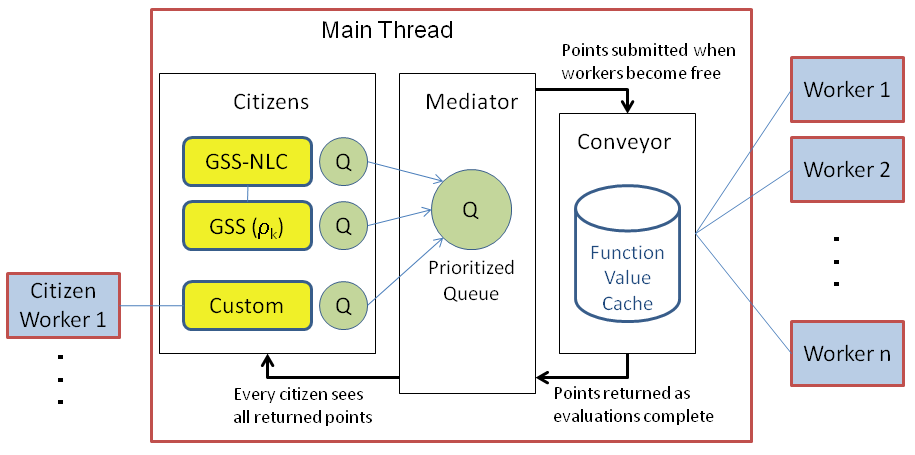
\includegraphics[width=5.8in]{BlockDiagram.png}
  \vspace{-5mm}
  \caption{HOPSPACK architecture diagram.}
  \label{fig:block-diagram}
\end{figure}

The Mediator runs a main processing loop until deciding that HOPSPACK should
stop.
Each Mediator iteration assembles trial point requests from all Citizens and
passes them to the Conveyor.  The Conveyor checks if new points can be fulfilled
from a cache, and sends the rest to idle workers for evaluation.  Two caches
are checked: a primary Cache of completed evaluations, and a Pending Cache
that lists trial points currently assigned to evaluation workers.
The Conveyor collects results from workers that have completed and passes
these back to the Mediator.
Citizens are then given the full set of newly evaluated points.  They examine
values and submit new trial points, which starts the
next iteration.  Citizens can also spawn dynamic ``child citizens'' to solve
subproblems.

From a citizen's point of view trial points are evaluated asynchronously,
so requests are typically managed with an internal queue, as shown in
\FIGREF{fig:block-diagram}.
The citizen submits trial points and may receive evaluated results at any
future iteration.  Evaluated points follow the order given from the citizen's
queue of trial points.  The citizen has the opportunity to retract previously
submitted points if they are still waiting on the Conveyor (for example,
the GSS citizen will retract old unevaluated requests when a new ``best point''
is found).
The Mediator collects trial requests from each citizen into a single
queue, interleaving points based on citizen priorities.

\FIGREF{fig:block-diagram} shows three citizen instances running
simultaneously.  The top two are connected because the GSS-NLC instance
dynamically created the GSS instance to solve a subproblem.  The citizen
labeled DIRECT has a parallel processing worker because its algorithm requires
significant CPU time to process points.  The ``citizen worker'' allows the
Mediator loop to run more quickly, and thus avoids slowing down other citizens.

As coordinator of the ``town'' of citizens, the Mediator decides when to
stop HOPSPACK and what final solution to return.
Each citizen decides when it has converged to a solution point, as defined by
its own criteria.  If all citizens have converged not necessarily to the same
point), then the Mediator stops.  It reports the best feasible point that it
has seen, regardless of which citizen generated the point.
If a problem-specific stop rule is supplied (for example,
an {\tt Objective Target} value, see \PGREF{param:PD-objtgt}),
then the Mediator will stop as soon as it sees a point satisfying the criteria
(see \SECREF{substoptest}).
The Mediator will also stop execution if a defined resource limit is reached
(for instance, execution time or the total number of worker evaluations).

The Cache in \FIGREF{fig:block-diagram} is an important feature of
HOPSPACK that often improves performance of GSS and related algorithms.
The Cache remembers all points and values that have been evaluated.  If a new
trial point is sufficiently close to a cached value, then it reports the stored
value instead of making another evaluation.  The definition of ``closeness''
is controlled by the
{\tt Cache Comparison Tolerance} parameter~(\PGREF{param:MD-cachetol}).
The Cache can also write its contents to a file
({\tt Cache Output File},~\PGREF{param:MD-cacheoutfile}), and load from
a file ({\tt Cache Input File},~\PGREF{param:MD-cacheinfile})
when HOPSPACK initializes.
This feature allows HOPSPACK to be interrupted without losing work.
As an interesting exercise, try solving a problem and saving the cache to a file,
and then solving again after initializing from the cache file.
If the Mediator is instructed to use
{\tt Synchronous Evaluations}~(\PGREF{param:MD-synch}), then the problem
will solve completely from cached information.
If not synchronous then there may be a few new iterations that choose different
directions, but the citizen should quickly build up a cache that can
solve without any evaluations.

Workers run copies of the application to collect objective and nonlinear
constraint values at trial points.  Each worker runs a HOPSPACK Evaluator
instance, which typically calls the application as a separate process for
each trial point.  See \SECREF{sec:calleval} for details on how an application
is called.
The workers on the right side of \FIGREF{fig:block-diagram} run in
parallel under direction of the Conveyor.  The Conveyor uses an Executor
subclass, specialized either for MPI or multithreaded (MT) operation, to
coordinate workers.
\FIGREF{fig:evalMPI} shows an example of the worker partitioning for
HOPSPACK using MPI on three nodes, and \FIGREF{fig:evalMT} shows an
example of worker partitioning for HOPSPACK using multithreading on a
quad-core machine.


MPI and MT are complementary methods of obtaining parallel
performance.  MPI-based HOPSPACK can solve problems on computing clusters with
tens of thousands of nodes, while MT exploits the multi-core capacity of
a single machine.  MT binaries are available for most platforms, but 
MPI requires recompiling HOPSPACK source code with an
MPI-aware compiler.  


\clearpage
\begin{figure}[!h]
  \begin{center}
    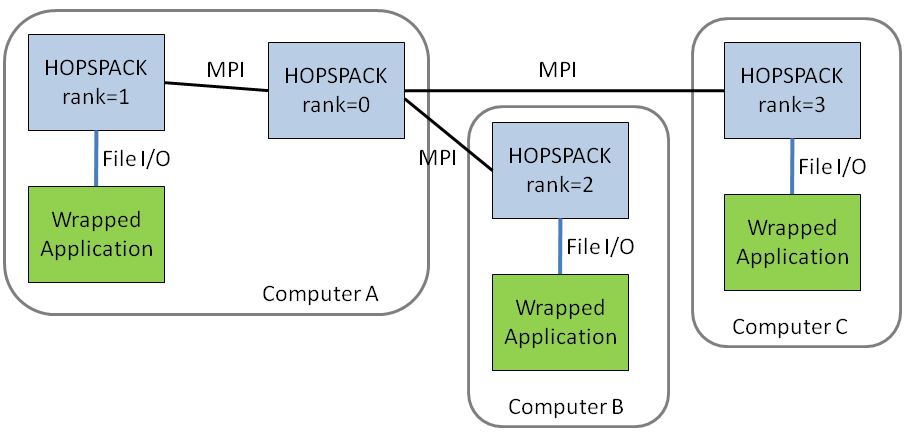
\includegraphics[width=5.0in]{EvalWithMpiClipped.png}
  \end{center}
  \vspace{-5mm}
  \caption{HOPSPACK communication using MPI.}
  \label{fig:evalMPI}
\end{figure}

\vspace{-11pt}
\noindent
In this example three copies of the application run in parallel
on three different computers.  Four MPI nodes are employed.
Evaluator nodes (rank 1, 2, 3) make system calls to the application,
and the main node (rank 0) runs the HOPSPACK Executor to control evaluations. 
The Mediator and Citizen solvers also run on the main node.
Execution may be faster if the main node can be placed on a separate computer.


% ADD SPACE TO LOOK BETTER, AND SO THE FIGURES CONSUME THE WHOLE PAGE.
% PUTTING \clearpage AT THE BOTTOM IS NOT THE SAME.
\vspace{11pt}
\vspace{11pt}
\vspace{11pt}


\begin{figure}[!h]
  \begin{center}
    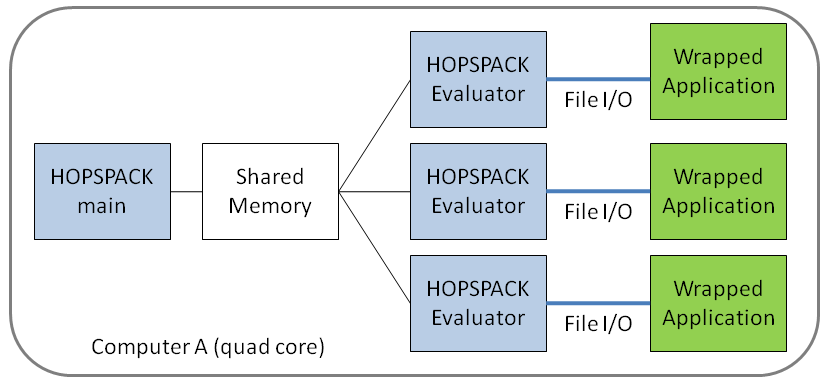
\includegraphics[width=5.0in]{EvalWithMtClipped.png}
  \end{center}
  \vspace{-5mm}
  \caption{HOPSPACK communication using multithreading.}
  \label{fig:evalMT}
\end{figure}

\vspace{-11pt}
\noindent
In this example three copies of the application run in parallel
as different processes on the same machine.  Four threads run in
the HOPSPACK process.
Evaluator threads make system calls to the application, and a fourth
thread runs the Executor to control evaluations.
The Mediator and Citizen solvers also run on the main thread.
Execution may be faster if additional cores are available for the application
instances.


%%%%%%%%%%%%%%%%%%%%
\subsection{Stopping Tests}
\label{substoptest}

The Mediator decides when to stop HOPSPACK and what to return as the best point
found.  The Mediator examines all evaluated points, regardless of which solver
submitted it, and keeps the best according to criteria discussed below.
HOPSPACK stops if any of the following conditions are met:
\begin{itemize}
  \item  All Citizen solvers are finished.
  \item  The total number of evaluations exceeds parameter
         {\tt Maximum Evaluations}~(\PGREF{param:MD-maxeval}).
         The default value of this parameter imposes no limit on evaluations.
  \item  The best point is feasible and satisfies an objective target set
         by the user.  Parameters
         {\tt Objective Target}~(\PGREF{param:PD-objtgt}) and
         {\tt Objective Percent Error}~(\PGREF{param:PD-objpcnt}) are
         used to set target values.  This is only useful if a practical value
         for the objective function is known.
\end{itemize}

A trial point is feasible if it satisfies the bound constraints, linear
constraints, and nonlinear constraints defined for the optimization problem.
Different tolerances are applied for each type of constraint:
\begin{INDENTdescription}
  \item[Bound constraints.]
    Variables are feasible if they satisfy the bound constraint exactly.
  \item[Linear constraints.]
    Linear equalities and inequalities are satisfied if within a tolerance set
    by parameter {\tt Active Tolerance} in the ``Linear Constraints'' sublist
    (\PGREF{param:LC-acttol}).  Computations are made in scaled coordinates
    (see {\tt Scaling}~(\PGREF{param:PD-scaling})) and normalized using
    the $L_2$ norm of the variables and the constraint.
  \item[Nonlinear constraints.]
    Nonlinear equalities and inequalities are satifisfied within a tolerance
    set by parameter {\tt Nonlinear Active Tolerance} in the
    ``Problem Definitions'' sublist (\PGREF{param:PD-nacttol}).
    Computations are not scaled.
\end{INDENTdescription}

The Mediator is responsible for choosing the best point that is output when
HOPSPACK finishes.  This is usually the same ``best point'' found by GSS
and other solvers, but not always.  The Mediator first seeks a point that
passes the feasibility tests described above.  If a feasible point has not
been found, then the least infeasible is ``best'', as measured by the
unscaled $L_{\infty}$ norm of the constraint vector.  If a feasible point has
been found, then a ``better'' point must pass the feasibility test and improve
on the objective value.
Source code is located in {\sf HOPSPACK\_Mediator.cpp} in the method
{\tt Mediator::updateBestPoint\_()}.

%TBD multiple objectives?


%%%%%%%%%%%%%%%%%%%%
\subsection{GSS Overview}
\label{subgss}

Generating Set Search (GSS) in HOPSPACK is an asynchronous implementation
of pattern search ideas.  An excellent review of pattern search methods
and convergence theory is in \cite{SIAMRev-KoLeTo03}.
GSS with linear constraints is explained in \cite{GSS-GrKoLe08} and
\cite{GSS-KoLeTo06},
and GSS with nonlinear constraints in \cite{GSS-GrKoSAND07}.
This overview will provide only a brief outline of the GSS algorithm.

The most basic GSS method addresses problems with continuous variables and
only bound constraints.  GSS begins with an arbitrary initial point and
iterates until stopped.  Each iteration generates a trial point along the
positive and negative direction of each coordinate axis.  The set of search
directions are centered on the current best point (called the ``parent'' point)
and initially extend a certain fixed distance.
If one of these trial points improves
on the parent, then it becomes the new best point for the next round.
If a trial point does worse, then the step size in that direction is reduced
to generate a replacement trial point.  GSS ends when the step length becomes
sufficiently short in every direction emanating from the current best point.
Details of this process are explained in the references and in
\SECREF{subconfig:GS}.  In particular, parameter
{\tt Step Tolerance}~(\PGREF{param:GS-steptol}) determines the length of
a ``sufficiently short'' step that stops the algorithm.

The HOPSPACK implementation of GSS is asynchronous in the sense that iterations
do not wait for all trial points in a direction set to be evaluated.  The
algorithm takes action on any partial set of results and is therefore ideal
for parallel architectures.  Convergence properties are no different for the
asynchronous algorithm.  An asynchronous implementation is especially tolerant
of applications whose run time varies based on the trial point.  For example,
if certain input regions require much more computation time in the application,
GSS will make progress in regions that run fast while waiting for the slower
points to evaluate.

GSS can respond to ``oracle'' inputs provided by another solver.  If an
evaluation result is better than the current GSS best point, then GSS will
adopt this as the new best point and begin searching around it.
The feature is controlled by parameter
{\tt Ignore Other Points}~(\PGREF{param:GS-ignore}).

The addition of linear constraints requires the set of directions to conform
with active constraints.  GSS honors linear equality constraints
at all times, and designates linear inequalities as active if the parent
point is within a distance {\tt Epsilon Max}~(\PGREF{param:GS-epsmax}).
Trial points are always feasible with respect to linear constraints.
To speed up the search, GSS can guess whether a nearby linear inequality
is active and ``snap'' a trial point to the bound; this feature is controlled
by parameters {\tt Snap To Boundary}~(\PGREF{param:GS-snap}) and
{\tt Snap Distance}~(\PGREF{param:GS-snapdist}).

{\bf GSS-NLC.}
The basic GSS solver handles continuous variables with bounds and linear
constraints, and was available in APPSPACK 5.0.  GSS is extended in HOPSPACK
to handle nonlinear constraints in a citizen called GSS-NLC.
The algorithm treats violations of nonlinear
constraints with a penalty term in the objective \cite{GSS-GrKoSAND07}.
An outer loop of iterations sets the weight of the penalty term and starts
a basic GSS citizen to solve a version of the problem without nonlinear
constraints.  This continues until the subproblem returns a feasible point
that also satisfies the {\tt Step Tolerance}~(\PGREF{param:GS-steptol}).
The inner loop of points generated by the subproblem solver behaves the same
as a basic GSS citizen except its initial point and stop criteria are set
by the GSS-NLC outer solver.

Performance of GSS-NLC can be heavily influenced by the penalty term and its
weight (the weight is also referred to as the penalty parameter).
Configuration parameters described in \SECREF{subconfig:GSN} provide
more information.
The values of {\tt Final Step Tolerance}~(\PGREF{param:GSN-finalstep}),
{\tt Nonlinear Active Tolerance}~(\PGREF{param:PD-nacttol}),
and {\tt Penalty Parameter Increase}~(\PGREF{param:GSN-penincrease})
are particularly important.  In general the penalty parameter should be increased
rapidly to force feasibility, but on some problems a slightly infeasible path
will reach an active nonlinear inequality constraint faster; in this case
the penalty parameter should be increased slowly.  The user is encouraged
to experiment.

The HOPSPACK framework allows a GSS-NLC citizen to create and manage subproblems
as separate GSS citizens.  This is shown schematically in
Figure~\ref{fig:block-diagram}, where a GSS-NLC citizen is connected with
a citizen labelled GSS($\rho_k$) (the penalty parameter of the subproblem
is $\rho_k$).  Subproblems run like any other citizen, but when they finish
their result is returned to the parent citizen that created them.
This idea is leveraged to extend GSS for problems with integer variables
and multiple start points.


\begin{figure}[!ht]
  \begin{center}
    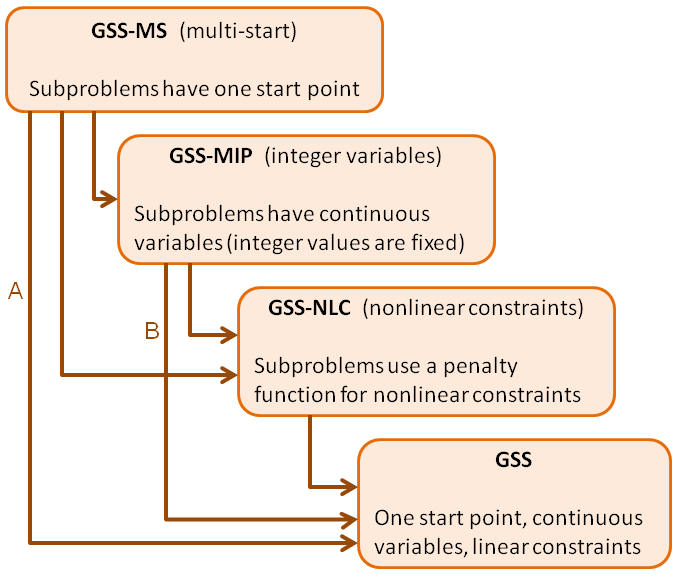
\includegraphics[width=5.0in]{GssHierarchyDiagram.png}
    \vspace{-5mm}
  \caption{Hierarchy of GSS algorithms,
           showing how complicated problems are decomposed into
           simpler subproblems.
           Arrows ``A'' and ``B'' are referenced in the text.
          }
  \label{fig:gss-hier}
  \end{center}
\end{figure}

\FIGREF{fig:gss-hier} shows how a notional family of GSS algorithms can address
a hierarchy of problem types.  (The current HOPSPACK release does not include
GSS-MIP, and GSS-MS has only partial functionality.)
Complicated problems at the top follow one or more
arrows to reach the basic GSS building block at the bottom.  An arrow indicates
that a problem is transformed into a sequence of simpler subproblems.
For example, path {\it A} shows that a multi-start problem with continuous
variables and linear constraints is solved by creating GSS subproblems, each
with a different starting point.  The parent GSS-MS collects subproblem results
and generates new start points until finished.
Path {\it B} shows that a problem with integer-valued variables and linear
constraints can be solved by creating GSS subproblems, each treating integer
variables as fixed to a specific integer value.  The parent GSS-MIP follows
a branching tree or other combinatorial strategy to decide how to fix
integer variables in each subproblem.
In the most complex case, a problem with multiple start points,
integer variables, and nonlinear constraints would cascade from GSS-MS
to GSS-MIP to GSS-NLC to GSS, creating subproblems of every type.

%%%%%%%%%%%%%%%%%%%%%%%%%%%%%%%%%%%%%%%%%%%%%%%%%%%%%%%%%%%%%%%%%%%%%%
\section{Config Parameters}
\label{sec:params}

Execution of HOPSPACK is controlled by a number of configuration parameters.
The user provides a text file containing parameters and passes the file name
on the command line.  HOPSPACK reads the file, parses parameter values,
and stores them for use during execution.
Most parameters have default values, but an input file is always required
to define the optimization problem and how it is evaluated.

As an example, consider solving
\[
  \begin{array}{cc}
    \min
      & (x_1 - 10)^2 + (x_2 - 10)^2 + (x_3 - 10)^2 + (x_4 - 10)^2  \\
    \vspace{-0.1in}  \\
    \mbox{subject to}
      & \begin{array}{rcrcr}
              &      & -x_1 - x_2 - x_3 - x_4 & \geq & -10    \\
           -1 & \geq &  x_1 - x_2 + x_3 - x_4                 \\
              &      & 2x_1 \hspace{5mm} +2x_3 -7x_4 & =    &  3  \\
      \end{array}  \\
      & \hspace{1.0in}
        10 \; \geq \; x_i \; \geq \; -10  \qquad i = 1, \ldots, 4
  \end{array}
\]
This problem is provided in the directory {\sf examples/2-linear-constraints},
where there is more documentation.
The input lines below are sufficient to define and solve the problem on HOPSPACK:
\begin{verbatim}
    @ "Problem Definition"
      "Number Unknowns" int 4                    # Number of variables
      "Upper Bounds" vector 4  10  10  10  10    # Variable upper bounds
      "Lower Bounds" vector 4 -10 -10 -10 -10    # Variable lower bounds
      "Initial X"    vector 4  -1   1  -1  -1    # Initial point
    @@
    @ "Linear Constraints"
      "Inequality Matrix" matrix 2 4             # 2 ineq, 4 variables
       -1 -1 -1 -1
        1 -1  1 -1
      "Inequality Lower" vector 2  -10 DNE       # Lower bounds on 2 ineqs
      "Inequality Upper" vector 2  DNE  -1       # Upper bounds on 2 ineqs
      "Equality Matrix" matrix 1 4               # 1 equality, 4 variables
       2.0  0  2.0  -0.7e+1
      "Equality Bounds" vector 1 3               # Right-hand side of eqs
    @@
    @ "Evaluator"                                # Program computing the obj
      "Executable Name" string "linear_constraints"
    @@
    @ "Mediator" 
      "Citizen Count" int 1                      # One citizen to start
    @@
    @ "Citizen 1"                                # Citizen name
      "Type" string "GSS"                        # Generalized Set Search
    @@
\end{verbatim}

As the example illustrates, parameters are organized into sublists that begin
with the {\tt @} character and a keyword name; for example,
{\tt @ "Problem Definition"}.  Sublists end with a line containing {\tt @@}.
Sublists can appear in any order.

Within a sublist are one or more parameters, each on a separate line.
Parameters can appear in any order within a sublist.  Parameter names are
scoped within a sublist, so if the same parameter name appears in two
sublists, it is actually two separate parameters with separate values.
Each line begins with the parameter name (a case-sensitive string), the type
of the parameter ({\tt int}, {\tt double}, etc.), and then the value.
The file can contain empty lines, leading whitespace, and comments beginning
with the {\tt \#} character.

\begin{itemize}
\item
String, integer, and double precision parameters are specified as follows:
\begin{verbatim}
      "String Parameter Name" string "string value"
      "Integer Parameter Name" int integer_value
      "Double Parameter Name" double double_value
\end{verbatim}
The double precision value can be in floating point or scientific format.
HOPSPACK also accepts the string ``{\tt DNE}'' for a double precision value,
which indicates the value ``does not exist''.  For instance, in the example above
{\tt DNE} is used to show the first inequality constraint has no upper bound.

\item
Boolean values are specified as follows:
\begin{verbatim}
      "Boolean Parameter Name" bool value
\end{verbatim}
The value is the word ``true'' or ``false'', without quotes, or one of the
equivalent words ``TRUE'', ``True'', ``T'' (similarly, for ``false'').

\item
Vector parameters are specified with a length (N) and then double precision
values, all on one line:
\begin{verbatim}
      "Vector Parameter Name" vector N double_1 ... double_N
\end{verbatim}

\item
Matrix parameters are specified with a number of rows (M) and columns (N).
Double precision values for each row are given on consecutive lines:
\begin{verbatim}
      "Matrix Parameter Name" matrix M N
        double_1,1 ... double_1,N
        double_2,1 ... double_2,N
                 ...
        double_M,1 ... double_M,N
\end{verbatim}

\item
A special character vector parameter is used to specify variable types.
It is a vector of single-letter characters:
\begin{verbatim}
      "Character Vector Parameter Name" charvec N char_1 ... char_N
\end{verbatim}

\end{itemize}

The next section (\ref{subconfig:DEFINITION}) describes the
assumptions made when formulating an optimization problem. A
quick reference guide to all the parameters is provided in
\SECREF{subconfig:QUICKREF}. The remaining sections
describe each parameter in HOPSPACK, grouped by sublist.


%%%%%%%%%%%%%%%%%%%%
\subsection{Defining the Optimization Problem}
\label{subconfig:DEFINITION}

Certain conventions are assumed when defining an optimization problem for
HOPSPACK.  The main points are described below.  Documentation of the
configuration parameters should also be consulted, especially the
``Problem Definition'' sublist (\SECREF{subconfig:PD}) and
the ``Linear Constraints'' sublist (\SECREF{subconfig:LC}).


\begin{itemize}

\item
Variables appear in an arbitrary order determined by the user, but that order
must be maintained when listing upper and lower bounds, variable types,
scaling factors, and any initial start point.

\item
If the objective cannot be evaluated at a point, then the application should
return the string ``{\tt DNE}'' to indicate the value does not exist.
Also return {\tt DNE} for any nonlinear constraints that cannot be evaluated
at a point.

\item
Linear equalities and inequalities are separated using different parameters
(see \SECREF{subconfig:LC}).  Constraints within each set
appear in an arbitrary order determined by the user, but that order must be
maintained when listing the matrix coefficients and bounds.  A single inequality
can have a lower and upper bound, or just one bound.

\item
Nonlinear equalities and inequalities are separated.  Constraints within each set
appear in an arbitrary order determined by the user, but that order must be
maintained when returning evaluation values or defining values at an initial
start point.
Nonlinear equalities should be defined to equal zero; i.e., a value of zero
at $x$ indicates the equality is satisfied:
\[
  c_{\cal E}(x) = 0 .
\]
Nonlinear inequalities should be defined as greater than zero:
\[
  c_{\cal I}(x) \geq 0 .
\]
Hence, a negative value at $x$ indicates that an inequality is violated,
and a nonnegative value indicates feasibility.
A nonlinear inequality with an upper and lower bound should be written as
two inequalities; for example,
\[
  \begin{array}{ccc}
     8 \; \geq \; x^2 + y^2 \; \geq \; 5
    & \rightarrow
    & \left\{ \begin{array}{rcl}
                8 - x^2 - y^2 & \geq & 0  \\
                x^2 + y^2 - 5 & \geq & 0
              \end{array}
      \right.
  \end{array}
\]

\end{itemize}


%%%%%%%%%%%%%%%%%%%%
\clearpage
\subsection{Quick Reference for Config Parameters}
\label{subconfig:QUICKREF}

The tables below list all configuration parameters in alphabetical order,
grouped by sublist.

\begin{tabbing}
  xx \= xxxxxxxxxxxxxxxxxxxxxxxxxxxxxxx \= xxxxxxxx \= \kill
  \>{\bf Problem Definition} sublist (\SECREF{subconfig:PD})  \\
  \>{\it Parameter Name}               \>{\it Type}
      \>{\it Default Value}  \\

  \>Display                            (\PGREF{param:PD-display})
      \>{\tt int}
      \>{\tt 0} (no display of problem definition)  \\
  \>Initial F                          (\PGREF{param:PD-initf})
      \>{\tt vector}
      \>{\tt DNE} (no initial values)  \\
  \>Initial Nonlinear Eqs              (\PGREF{param:PD-initeqs})
      \>{\tt vector}
      \>{\tt DNE} (no initial values)  \\
  \>Initial Nonlinear Ineqs            (\PGREF{param:PD-initineqs})
      \>{\tt vector}
      \>{\tt DNE} (no initial values)  \\
  \>Initial X                          (\PGREF{param:PD-initx})
      \>{\tt vector}
      \>no initial point  \\
  \>Lower Bounds                       (\PGREF{param:PD-lbnd})
      \>{\tt vector}
      \>no lower bounds (all equal {\tt DNE})  \\
  \>Nonlinear Active Tolerance         (\PGREF{param:PD-nacttol})
      \>{\tt double}
      \> {\tt 1.0e-7}  \\
  \>Number Nonlinear Eqs               (\PGREF{param:PD-numeqs})
      \>{\tt int}
      \>{\tt 0}  \\
  \>Number Nonlinear Ineqs             (\PGREF{param:PD-numineqs})
      \>{\tt int}
      \>{\tt 0}  \\
  \>Number Objectives                  (\PGREF{param:PD-numobjs})
      \>{\tt int}
      \>{\tt 1}  \\
  \>Number Unknowns                    (\PGREF{param:PD-numunks})
      \>{\tt int}
      \> none (parameter is required)  \\
  \>Objective Percent Error            (\PGREF{param:PD-objpcnt})
      \>{\tt double}
      \>{\tt DNE} (no stop test based on percent error)  \\
  \>Objective Target                   (\PGREF{param:PD-objtgt})
      \>{\tt double}
      \>{\tt DNE} (no target)  \\
  \>Objective Type                     (\PGREF{param:PD-objtype})
      \>{\tt string}
      \>{\tt "Minimize"}  \\
  \>Scaling                            (\PGREF{param:PD-scaling})
      \>{\tt vector}
      \>automatic scaling if possible  \\
  \>Upper Bounds                       (\PGREF{param:PD-ubnd})
      \>{\tt vector}
      \>no upper bounds (all equal {\tt DNE})  \\
  \>Variable Types                     (\PGREF{param:PD-vartypes})
      \>{\tt charvec}
      \>all variables continuous
\end{tabbing}

\begin{tabbing}
  xx \= xxxxxxxxxxxxxxxxxxxxxxxxxxxxxxx \= xxxxxxxx \= \kill
  \>{\bf Linear Constraints} sublist (\SECREF{subconfig:LC})  \\
  \>{\it Parameter Name}               \>{\it Type}
      \>{\it Default Value}  \\

  \>Active Tolerance                   (\PGREF{param:LC-acttol})
      \>{\tt double}
%TBD      \> 4 * machine epsilon ($\approx 8.9 \times 10^{-16}$)  \\
      \> {\tt 1.0e-12}  \\
  \>Display                            (\PGREF{param:LC-display})
      \>{\tt int}
      \> {\tt 0} (no display of constraints)  \\
  \>Equality Bounds                    (\PGREF{param:LC-eqbnds})
      \>{\tt vector}
      \> no equality constraints  \\
  \>Equality Matrix                    (\PGREF{param:LC-eqmat})
      \>{\tt matrix}
      \> no equality constraints  \\
  \>Inequality Lower                   (\PGREF{param:LC-ineql})
      \>{\tt vector}
      \> no inequality constraints  \\
  \>Inequality Matrix                  (\PGREF{param:LC-ineqmat})
      \>{\tt matrix}
      \> no inequality constraints  \\
  \>Inequality Upper                   (\PGREF{param:LC-inequ})
      \>{\tt vector}
      \> no inequality constraints
\end{tabbing}

\begin{tabbing}
  xx \= xxxxxxxxxxxxxxxxxxxxxxxxxxxxxxx \= xxxxxxxx \= \kill
  \>{\bf Evaluator} sublist (\SECREF{subconfig:EV})  \\
  \>{\it Parameter Name}               \>{\it Type}
      \>{\it Default Value}  \\

  \>Debug Eval Worker                  (\PGREF{param:EV-debug})
      \>{\tt bool}
      \>{\tt false}  \\
  \>Evaluator Type                     (\PGREF{param:EV-type})
      \>{\tt string}
      \>{\tt "System Call"}  \\
  \>Executable Name                    (\PGREF{param:EV-execname})
      \>{\tt string}
      \>{\tt "a.out"}  \\
  \>File Precision                     (\PGREF{param:EV-prec})
      \>{\tt int}
      \>{\tt 14}  \\
  \>Input Prefix                       (\PGREF{param:EV-inprefix})
      \>{\tt string}
      \>{\tt "input"}  \\
  \>Output Prefix                      (\PGREF{param:EV-outprefix})
      \>{\tt string}
      \>{\tt "output"}  \\
  \>Save IO Files                      (\PGREF{param:EV-savefiles})
      \>{\tt bool}
      \>{\tt false}
\end{tabbing}

\begin{tabbing}
  xx \= xxxxxxxxxxxxxxxxxxxxxxxxxxxxxxx \= xxxxxxxx \= \kill
  \>{\bf Mediator} sublist (\SECREF{subconfig:ME})  \\
  \>{\it Parameter Name}               \>{\it Type}
      \>{\it Default Value}  \\

  \>Cache Comparison Tolerance         (\PGREF{param:MD-cachetol})
      \>{\tt double}
      \> 2 * machine epsilon ($\approx 4.4 \times 10^{-16}$)  \\
  \>Cache Enabled                      (\PGREF{param:MD-cacheenabled})
      \>{\tt bool}
      \>{\tt true}  \\
  \>Cache Input File                   (\PGREF{param:MD-cacheinfile})
      \>{\tt string}
      \>no input file  \\
  \>Cache Output File                  (\PGREF{param:MD-cacheoutfile})
      \>{\tt string}
      \>no output file  \\
  \>Cache Output Precision             (\PGREF{param:MD-cacheoutfileprec})
      \>{\tt int}
      \>{\tt 14}  \\
  \>Citizen Count                      (\PGREF{param:MD-ctzns})
      \>{\tt int}
      \>none (parameter is required)  \\
  \>Display                            (\PGREF{param:MD-display})
      \>{\tt int}
      \>{\tt 2}  \\
  \>Max Initial Eval Failures          (\PGREF{param:MD-maxinitfails})
      \>{\tt int}
      \>{\tt 5}  \\
  \>Maximum Evaluations                (\PGREF{param:MD-maxeval})
      \>{\tt int}
      \>{\tt -1} (unlimited)  \\
  \>Maximum Exchange Return            (\PGREF{param:MD-maxexch})
      \>{\tt int}
      \>{\tt 1000}  \\
  \>Minimum Exchange Return            (\PGREF{param:MD-minexch})
      \>{\tt int}
      \>{\tt 1}  \\
  \>Number Processors                  (\PGREF{param:MD-numproc})
      \>{\tt int}
      \> none (parameter required with MPI)  \\
  \>Number Threads                     (\PGREF{param:MD-numthreads})
      \>{\tt int}
      \> none (parameter required if multithreaded)  \\
  \>Precision                          (\PGREF{param:MD-prec})
      \>{\tt int}
      \>{\tt 3}  \\
  \>Reserved Citizen Workers           (\PGREF{param:MD-resctzns})
      \>{\tt int}
      \>{\tt 0}  \\
  \>Solution File                      (\PGREF{param:MD-solfile})
      \>{\tt string}
      \>no solution file  \\
  \>Solution File Precision            (\PGREF{param:MD-solfileprec})
      \>{\tt int}
      \>{\tt 14}  \\
  \>Synchronous Evaluations            (\PGREF{param:MD-synch})
      \>{\tt bool}
      \>{\tt false}
\end{tabbing}

\begin{tabbing}
  xx \= xxxxxxxxxxxxxxxxxxxxxxxxxxxxxxx \= xxxxxxxx \= \kill
  \>{\bf Citizen GSS} sublist (\SECREF{subconfig:GS})  \\
  \>{\it Parameter Name}               \>{\it Type}
      \>{\it Default Value}  \\

  \>Add Projected Compass              (\PGREF{param:GS-addcompass})
      \>{\tt bool}
      \>{\tt false}  \\
  \>Add Projected Normals              (\PGREF{param:GS-addnormals})
      \>{\tt bool}
      \>{\tt true}  \\
  \>Citizen Priority                   (\PGREF{param:GS-priority})
      \>{\tt int}
      \>{\tt 1} (highest priority)  \\
  \>Contraction Factor                 (\PGREF{param:GS-contract})
      \>{\tt double}
      \>{\tt 0.5}  \\
  \>Display                            (\PGREF{param:GS-display})
      \>{\tt int}
      \>{\tt 0} (no display of GSS operation)  \\
  \>Epsilon Max                        (\PGREF{param:GS-epsmax})
      \>{\tt double}
      \>{\tt 2 * Step Tolerance}  \\
  \>Ignore Other Points                (\PGREF{param:GS-ignore})
      \>{\tt bool}
      \>{\tt false}  \\
  \>Initial Step                       (\PGREF{param:GS-initstep})
      \>{\tt double}
      \>{\tt 1.0}  \\
  \>Maximum Evaluations                (\PGREF{param:GS-maxeval})
      \>{\tt int}
      \>{\tt -1} (unlimited)  \\
  \>Maximum Queue Size                 (\PGREF{param:GS-maxq})
      \>{\tt int}
      \>{\tt 0}  \\
  \>Minimum Step                       (\PGREF{param:GS-minstep})
      \>{\tt double}
      \>{\tt 2 * Step Tolerance}  \\
  \>Penalty Function                   (\PGREF{param:GS-penfn})
      \>{\tt string}
      \>{\tt "L2 Squared"}  \\
  \>Penalty Parameter                  (\PGREF{param:GS-penparam})
      \>{\tt double}
      \>{\tt 1.0}  \\
  \>Penalty Smoothing Value            (\PGREF{param:GS-pensmooth})
      \>{\tt double}
      \>{\tt 0.0}  \\
  \>Snap Distance                      (\PGREF{param:GS-snapdist})
      \>{\tt double}
      \>{\tt Step Tolerance / 2}  \\
  \>Snap To Boundary                   (\PGREF{param:GS-snap})
      \>{\tt bool}
      \>{\tt false}  \\
  \>Step Tolerance                     (\PGREF{param:GS-steptol})
      \>{\tt double}
      \>{\tt 0.01}  \\
  \>Sufficient Improvement Factor      (\PGREF{param:GS-suffimpr})
      \>{\tt double}
      \>{\tt 0.01}  \\
  \>Type                               (\PGREF{param:GS-type})
      \>{\tt string}
      \>{\tt "GSS"}  \\
  \>Use Random Order                   (\PGREF{param:GS-random})
      \>{\tt bool}
      \>{\tt true}
\end{tabbing}

\begin{tabbing}
  xx \= xxxxxxxxxxxxxxxxxxxxxxxxxxxxxxx \= xxxxxxxx \= \kill
  \>{\bf Citizen GSS-NLC} sublist (\SECREF{subconfig:GSN})  \\
  \>{\it Parameter Name}               \>{\it Type}
      \>{\it Default Value}  \\

  \>Display                            (\PGREF{param:GSN-display})
      \>{\tt int}
      \>{\tt 0} (no display of GSS-NLC operation)  \\
  \>Display Subproblem                 (\PGREF{param:GSN-displaysub})
      \>{\tt int}
      \>{\tt 0} (no display of subproblem operation)  \\
  \>Final Step Tolerance               (\PGREF{param:GSN-finalstep})
      \>{\tt double}
      \>{\tt 0.001}  \\
  \>Ignore Other Points                (\PGREF{param:GSN-ignore})
      \>{\tt bool}
      \>{\tt false}  \\
  \>Initial Step Tolerance             (\PGREF{param:GSN-initialstep})
      \>{\tt double}
      \>{\tt 0.1}  \\
  \>Maximum Evaluations                (\PGREF{param:GSN-maxeval})
      \>{\tt int}
      \>{\tt -1} (unlimited)  \\
  \>Max Subproblem Evaluations         (\PGREF{param:GSN-maxsubeval})
      \>{\tt int}
      \>{\tt -1} (unlimited)  \\
  \>Penalty Function                   (\PGREF{param:GSN-penfn})
      \>{\tt string}
      \>{\tt "L2 Squared"}  \\
  \>Penalty Parameter                  (\PGREF{param:GSN-penparam})
      \>{\tt double}
      \>{\tt 1.0}  \\
  \>Penalty Parameter Increase         (\PGREF{param:GSN-penincrease})
      \>{\tt double}
      \>{\tt 2.0}  \\
  \>Penalty Parameter Maximum          (\PGREF{param:GSN-penmax})
      \>{\tt double}
      \>{\tt 1.0e+8}  \\
  \>Penalty Smoothing Value            (\PGREF{param:GSN-pensmooth})
      \>{\tt double}
      \>{\tt 0.0}  \\
  \>Smoothing Value Decrease           (\PGREF{param:GSN-smoothdecrease})
      \>{\tt double}
      \>{\tt 0.5}  \\
  \>Smoothing Value Minimum            (\PGREF{param:GSN-smoothmin})
      \>{\tt double}
      \>{\tt 1.0e-5}  \\
  \>Step Tolerance Decrease            (\PGREF{param:GSN-steptoldecrease})
      \>{\tt double}
      \>{\tt 0.5}  \\
  \>Type                               (\PGREF{param:GSN-type})
      \>{\tt string}
      \>{\tt "GSS-NLC"}
\end{tabbing}


%%%%%%%%%%%%%%%%%%%%
\clearpage
\subsection{Problem Definition Sublist Parameters}
\label{subconfig:PD}

This sublist defines the optimization objective, the variables, bounds on
the variables, scaling factors for each variable, a starting point for algorithms
to use, and the number and type of nonlinear constraints.
The sublist has one required parameter:  {\tt Number Unknowns}.
All other parameters have default values that assume the problem is an
unconstrained minimization of continuous variables.

%----
\subparagraph{Number Unknowns.}  \label{param:PD-numunks}
Specifies the number of optimization variables in the problem, including
continuous and integer-valued unknowns.
The parameter value must be a positive integer.

\hspace{0.2in}
Type: {\tt int}

\hspace{0.2in}
Default: none (the parameter is required)

\hspace{0.2in}
Example: {\tt "Number Unknowns" int 4}
%----

%----
\subparagraph{Lower Bounds.}  \label{param:PD-lbnd}
Specifies a lower bound for each variable.  If a variable has
no lower bound, then use the value {\tt DNE} in that position of the vector.
It is possible, but not recommended, to define a simple variable bound as an
inequality in the ``Linear Constraints'' sublist.
The number of values supplied by the parameter must equal the number of unknowns.

\hspace{0.2in}
Type: {\tt vector}

\hspace{0.2in}
Default: no lower bounds (all values equal {\tt DNE})
%----

%----
\subparagraph{Upper Bounds.}  \label{param:PD-ubnd}
Specifies an upper bound for each variable.  If a variable has
no upper bound, then use the value {\tt DNE} in that position of the vector.
It is possible, but not recommended, to define a simple variable bound as an
inequality in the ``Linear Constraints'' sublist.
The number of values supplied by the parameter must equal the number of unknowns.

\hspace{0.2in}
Type: {\tt vector}

\hspace{0.2in}
Default: no upper bounds (all values equal {\tt DNE})
%----

%----
\subparagraph{Scaling.}  \label{param:PD-scaling}
Variables with widely different ranges can substantially slow the convergence
of GSS and other algorithms.  Scaling allows algorithms to correct for the
discrepancy, and is considered essential for good performance.

\noindent
The parameter states the expected range of each variable, in either absolute
or relative terms.  If no parameter is specified, then a default value of one
is used (i.e., all variables are scaled equally).
However, HOPSPACK insists that the problem define either scaling or upper
and lower bounds on each variable.  This ensures citizens have some information
about the range of variables for their algorithm; for example, GSS chooses
a default value for {\tt Initial Step}~(\PGREF{param:GS-initstep})
based on the scaling or variable bounds.

\noindent
The GSS algorithm makes many internal calculations in scaled coordinates, and
its behavior can change based on the scaling.  For example, the
{\tt Step Tolerance}~(\PGREF{param:GS-steptol}) determines when a local
solution is found.  If scaling is increased for a problem, then the step
tolerance may need to decrease in order to reach a solution with the same
accuracy.

\noindent
If the user has no information about variable scaling but is confident of the
upper and lower bounds, then often a reasonable guess for scaling is the
range of the variable:
\[
  \mbox{scale}_i = u_i - l_i
\]
The number of values supplied by the parameter must equal the number of unknowns.

\hspace{0.2in}
Type: {\tt vector}

\hspace{0.2in}
Default: automatic scaling if possible, else the parameter is required
%----

%----
\subparagraph{Variable Types.}  \label{param:PD-vartypes}
Specifies the type of each variable with a vector of character values.
Possible character codes are {\tt C} (or {\tt c}) for real-valued continuous
variables, {\tt I} (or {\tt i}) for integer-valued variables that can be
relaxed to continuous values, and {\tt O} (or {\tt o}) for ordinal
variables that can only take integer values.
Variables of type {\tt I} and {\tt O} are both integral at the solution, but
an application with type {\tt I} variables will accept continuous values;
for example, mixed integer programming problems that can be relaxed to
a continuous linear programming problem have variables of type {\tt I}.
Type {\tt O}, known as ordinal or categorical variables, require
integer values at all evaluations points.
The number of values supplied by the parameter must equal the number of unknowns.

\hspace{0.2in}
Type: {\tt charvec}

\hspace{0.2in}
Default: all variables continuous

\hspace{0.2in}
Example: {\tt "Variable Types" charvec 3  C C I}
%----

%----
\subparagraph{Number Objectives.}  \label{param:PD-numobjs}
Specifies the number of optimization objective functions.
A value of one indicates there is a single objective function.
A value of zero means there is no objective and the goal is to find a
feasible point.
A value greater than one indicates there are multiple objectives.

\hspace{0.2in}
Type: {\tt int}

\hspace{0.2in}
Default: {\tt 1}
%----

%----
\subparagraph{Objective Type.}  \label{param:PD-objtype}
Specifies the goal of the optimization, which must be one of the keywords
{\tt "Minimize"} or {\tt "Maximize"}.
The parameter is ignored if {\tt Number Objectives} is zero.

\hspace{0.2in}
Type: {\tt string}

\hspace{0.2in}
Default: {\tt "Minimize"}
%----

%----
\subparagraph{Objective Target.}  \label{param:PD-objtgt}
Specifies a satisfactory value for the objective function to reach.
If HOPSPACK finds a feasible point with an objective equal to or better than
the target value, then execution stops immediately.
If the {\tt Objective Type} parameter is {\tt "Minimize"},
then HOPSPACK stops when the objective value is less than or
equal to the target; if {\tt "Maximize"},
then it stops when the objective is greater than or equal to the target.
(Note:  in APPSPACK this parameter was called ``Known Global Minimum''.)

\noindent
In many problems the optimal value of the objective is not known.  In this case,
leave the parameter undefined.  HOPSPACK can still find a solution, but will
probably take more iterations compared to a known target, because it will
make extra evaluations to confirm that neighboring points are no better.

\noindent
Use the parameter {\tt Objective Percent Error} to instruct HOPSPACK to stop
when within a certain range of the target value.

\hspace{0.2in}
Type: {\tt double}

\hspace{0.2in}
Default: {\tt DNE} (no target)
%----

%----
\subparagraph{Objective Percent Error.}  \label{param:PD-objpcnt}
Specifies a desired value for the objective function to reach,
in terms of parameter {\tt Objective Target}.  Suppose the current objective
value is $f$ and the target value is $f_T$.  If $f$ reaches or exceeds the
target, then HOPSPACK stops, as explained in the description of parameter
{\tt Objective Target}.  If $f$ does not reach the target but is within a
percentage of it as defined in the equation below, then HOPSPACK stops.
Pseudocode for the combined stop test follows:
\begin{tabbing}
  xxxxxxxx \= xxxxxxxxxxxxxxxxxxxxxxxxxxxxxxxxxxxxxxxxxxxxxxxxxx \= \kill
     \> If $f$ reaches or exceeds {\tt Objective Target}
        \> Then stop  \\
     \> If $\; 100 \times
                \displaystyle \frac{| f - f_T |}{\max \{ 10^{-4}, | f_T | \}}
             \; \leq \;$ {\tt Objective Percent Error}
        \> Then stop
\end{tabbing}
The parameter value cannot be negative.

\hspace{0.2in}
Type: {\tt double}

\hspace{0.2in}
Default: {\tt DNE} (no stop test based on percent error)

\hspace{0.2in}
Example: {\tt "Objective Percent Error" double 2.5} (stop if within 2.5\%)
%----

%----
\subparagraph{Number Nonlinear Eqs.}  \label{param:PD-numeqs}
Specifies the number of nonlinear equality constraints in the problem.
Nonlinear equalities are defined in the form $c(x) = 0$, so a value of zero
indicates feasibility.

\hspace{0.2in}
Type: {\tt int}

\hspace{0.2in}
Default: {\tt 0}
%----

%----
\subparagraph{Number Nonlinear Ineqs.}  \label{param:PD-numineqs}
Specifies the number of nonlinear inequality constraints in the problem.
Nonlinear inequalities are defined in the form $c(x) \geq 0$, so a negative
value indicates the constraint is violated.

\hspace{0.2in}
Type: {\tt int}

\hspace{0.2in}
Default: {\tt 0}
%----

%----
\subparagraph{Nonlinear Active Tolerance.}  \label{param:PD-nacttol}
Specifies the maximum violation beyond which a nonlinear equality or inequality
constraint is considered active.  For example, if an equality constraint
evaluates to a value larger than the tolerance, then the point is interpreted
to be infeasible.
Note that the nonlinear tolerance is defined and treated differently
than the {\tt Active Tolerance} parameter
in the ``Linear Constraints'' sublist (\PGREF{param:LC-acttol}).

\hspace{0.2in}
Type: {\tt double}

\hspace{0.2in}
Default: {\tt 1.0e-7} ($10^{-7}$)
%----

%----
\subparagraph{Initial X.}  \label{param:PD-initx}
Initial point for optimization to begin at.  If any variable violates its
upper or lower bound, then it is moved to the bound to become feasible.
If the initial point violates linear constraints, then a least squares
subproblem is automatically solved to project it onto the constraints,
providing a feasible initial point.
If an initial point is not defined, then each citizen is at liberty to define
a default initial point.
The number of values supplied by the parameter must equal the number of unknowns.

\hspace{0.2in}
Type: {\tt vector}

\hspace{0.2in}
Default: no initial point
%----

%----
\subparagraph{Initial F.}  \label{param:PD-initf}
Provides known objective values at the initial point specified
by parameter {\tt Initial X}.  If no initial point is given, or if the
point is moved by HOPSPACK to satisfy constraints, then this parameter is
ignored.
If parameter {\tt Initial X} is given and this parameter is not, then
HOPSPACK will evaluate the initial point before any other trial points.

\hspace{0.2in}
Type: {\tt vector} (initial objective values)

\hspace{0.2in}
Default: values not known
%----

%----
\subparagraph{Initial Nonlinear Eqs.}  \label{param:PD-initeqs}
Provides known values for all nonlinear equality constraints at the initial
point specified by parameter {\tt Initial X}.
Nonlinear equalities are defined in the form $c(x) = 0$, so a value of zero
indicates feasibility.
If no initial point is given,
or if the point is moved by HOPSPACK to satisfy constraints, then this parameter
is ignored.
If the problem has nonlinear equalities, parameter {\tt Initial X} is given
and this parameter is not,
then HOPSPACK will evaluate the initial point before any other trial points.
The number of values supplied by the parameter must equal the value of
{\tt Number Nonlinear Eqs}.

\hspace{0.2in}
Type: {\tt vector} (initial equality constraint values)

\hspace{0.2in}
Default: values not known
%----

%----
\subparagraph{Initial Nonlinear Ineqs.}  \label{param:PD-initineqs}
Provides known values for all nonlinear inequality constraints at the initial
point specified by parameter {\tt Initial X}.
Nonlinear inequalities are defined in the form $c(x) \geq 0$, so a negative
value indicates the constraint is violated.
If no initial point is given,
or if the point is moved by HOPSPACK to satisfy constraints, then this parameter
is ignored.
If the problem has nonlinear inequalities, parameter {\tt Initial X} is given
and this parameter is not,
then HOPSPACK will evaluate the initial point before any other trial points.
The number of values supplied by the parameter must equal the value of
{\tt Number Nonlinear Ineqs}.

\hspace{0.2in}
Type: {\tt vector} (initial inequality constraint values)

\hspace{0.2in}
Default: values not known
%----

%----
\subparagraph{Display.}  \label{param:PD-display}
Specifies whether to print the problem definition to the console.
Printing of the problem definition can happen at the start of HOPSPACK execution,
and when the GSS citizen initializes.  Possible values are:
\begin{tabbing}
  xxxxxxxx \= xx \= \kill
     \> {\tt 0} \> display nothing \\
     \> {\tt 1} \> display problem summary  \\
     \> {\tt 2} \> display all details, including bounds and type of
                   each variable
\end{tabbing}

\hspace{0.2in}
Type: {\tt int}

\hspace{0.2in}
Default: {\tt 0} (display nothing)
%----


%%%%%%%%%%%%%%%%%%%%
\subsection{Linear Constraints Sublist Parameters}
\label{subconfig:LC}

This sublist defines linear equality and inequality constraints in the problem,
and a tolerance for determining when a constraint is active.
The sublist can be omitted if the problem has no linear constraints.
Simple bounds on a single variable should be defined in the
``Problem Definition'' sublist (\SECREF{subconfig:PD}).

%----
\subparagraph{Equality Bounds.}  \label{param:LC-eqbnds}
Provides the right-hand side for all linear equality constraints.
The order of values matches the order of the rows in {\tt Equality Matrix}.
See the example at the beginning of \SECREF{sec:params}.

\hspace{0.2in}
Type: {\tt vector}

\hspace{0.2in}
Default: no equality constraints
%----

%----
\subparagraph{Equality Matrix.}  \label{param:LC-eqmat}
Provides the left-hand side coefficients for all linear equality
constraints.  The order of matrix rows matches the order of the values
in {\tt Equality Bounds}.
The number of matrix columns must equal the number of unknowns.
Coefficients are listed in dense notation; that is, a zero value must be
given for any missing variable terms.
See the example at the beginning of \SECREF{sec:params}.

\hspace{0.2in}
Type: {\tt matrix}

\hspace{0.2in}
Default: no equality constraints
%----

%----
\subparagraph{Inequality Lower.}  \label{param:LC-ineql}
Provides the lower bound for all linear inequality constraints.
The order of values matches the order of the rows in {\tt Inequality Matrix}.
If an inequality has no lower bound, then use the value {\tt DNE} in that
position of the vector.
See the example at the beginning of \SECREF{sec:params}.

\hspace{0.2in}
Type: {\tt vector}

\hspace{0.2in}
Default: no inequality constraints
%----

%----
\subparagraph{Inequality Upper.}  \label{param:LC-inequ}
Provides the upper bound for all linear inequality constraints.
The order of values matches the order of the rows in {\tt Inequality Matrix}.
If an inequality has no upper bound, then use the value {\tt DNE} in that
position of the vector.
See the example at the beginning of \SECREF{sec:params}.

\hspace{0.2in}
Type: {\tt vector}

\hspace{0.2in}
Default: no inequality constraints
%----

%----
\subparagraph{Inequality Matrix.}  \label{param:LC-ineqmat}
Provides the coefficients for all linear inequality constraints.
The order of matrix rows matches the order of the values in
{\tt Inequality Lower} and {\tt Inequality Upper}.
The number of matrix columns must equal the number of unknowns.
Coefficients are listed in dense notation; that is, a zero value must be
given for any missing variable terms.
See the example at the beginning of \SECREF{sec:params}.

\hspace{0.2in}
Type: {\tt matrix}

\hspace{0.2in}
Default: no inequality constraints
%----

%----
\subparagraph{Active Tolerance.}  \label{param:LC-acttol}
Specifies the distance over which an equality or inequality boundary is
considered active.  For example, a point located beyond the active tolerance
of a linear equality constraint is interpreted to be infeasible.
Several other HOPSPACK operations depend on the tolerance value:
the computation of a step length to the bounds
(see {\tt HOPSPACK\_LinConstr::maxStep()}),
the choice of a set of active constraints to ``snap'' onto
(see {\tt HOPSPACK\_LinConstr::formSnapSystem()}),
the threshold for declaring a constraint to be degenerate
(see {\tt HOPSPACK\_Matrix::nullspace()}),
the construction of normal and tangent cones for generating search
directions in the GSS citizen (see methods in {\tt HOPSPACK\_GssDirections}),
and the solution of a least squares subproblem to project infeasible trial
points onto the linear constraints
(see methods in {\tt HOPSPACK\_SolveLinConstrProj}).

\noindent
In most cases the active tolerance is applied against a scaled distance
to a constraint.  Therefore, if {\tt Scaling}~(\PGREF{param:PD-scaling})
is large for some variables, the active tolerance may need to increase
beyond its default value.

\noindent
Note that the linear tolerance is defined and treated differently
than the {\tt Nonlinear Active Tolerance} parameter
in the ``Problem Definition'' sublist (\PGREF{param:PD-nacttol}).

\noindent
The problem in {\sf examples/2-linear-constraints} illustrates the importance of
this parameter.  If the tolerance is made smaller than the default, then some
trial points computed by projection onto the constraints are judged to be
infeasible.  As an example, try changing the tolerance to
{\tt 4.0e-16} (exact results of this experiment depend on the machine
architecture).

\hspace{0.2in}
Type: {\tt double}

\hspace{0.2in}
Default: {\tt 1.0e-12} ($10^{-12}$)
%----

%----
\subparagraph{Display.}  \label{param:LC-display}
Specifies whether to print the linear constraints to the console.
Printing of the problem definition can happen at the start of HOPSPACK execution,
and when the GSS citizen initializes.  Possible values are:
\begin{tabbing}
  xxxxxxxx \= xx \= \kill
     \> {\tt 0} \> display nothing \\
     \> {\tt 1} \> display linear constraints summary  \\
     \> {\tt 2} \> display all details, including the constraint matrices
\end{tabbing}

\hspace{0.2in}
Type: {\tt int}

\hspace{0.2in}
Default: {\tt 0} (display nothing)
%----



%%%%%%%%%%%%%%%%%%%%
\subsection{Evaluator Sublist Parameters}
\label{subconfig:EV}

This sublist determines how functions are evaluated.
Every optimization problem must provide a way for HOPSPACK to compute its
objective and nonlinear constraints.
Read \SECREF{sec:calleval} for an explanation of how HOPSPACK invokes
an evaluation.

%----
\subparagraph{Evaluator Type.}  \label{param:EV-type}
Specifies the evaluator type with a special string value.
Possible values are {\tt "System Call"} and {\tt "AMPL Call"}.

\hspace{0.2in}
Type: {\tt string}

\hspace{0.2in}
Default: {\tt "System Call"}
%----

%----
\subparagraph{Executable Name.}  \label{param:EV-execname}
Specifies the name of an executable program that HOPSPACK calls to evaluate
optimization problem data at a trial point.  The program is passed certain
command line arguments and uses files to communicate inputs and outputs.
See \SECREF{sec:calleval} for information on writing the executable.

\noindent
This parameter is used only if the {\tt Evaluator Type} parameter is
{\tt"System Call"}.  Note the executable name should be a full path
if the user's {\tt PATH} environment variable does not include the
location of the executable.

\hspace{0.2in}
Type: {\tt string}

\hspace{0.2in}
Default: {\tt "a.out"}
%----

%----
\subparagraph{Input Prefix.}  \label{param:EV-inprefix}
Specifies the prefix of file names that are used to pass input data to the
executable program defined by parameter {\tt Executable Name}.
The full file name has the
form {\sf input\_prefix.NNN\_TT}, where {\sf NNN} is a unique integer
tag assigned to the trial point and {\sf TT} is the type of information
requested.

\noindent
This parameter is used only if the {\tt Evaluator Type} parameter is
{\tt"System Call"}.

\hspace{0.2in}
Type: {\tt string}

\hspace{0.2in}
Default: {\tt "input"}
%----

%----
\subparagraph{File Precision.}  \label{param:EV-prec}
Specifies the number of digits after the decimal point
for each floating point number written to the file named with parameter
{\tt Input Prefix}.

\noindent
This parameter is used only if the {\tt Evaluator Type} parameter is
{\tt"System Call"}.

\hspace{0.2in}
Type: {\tt int}

\hspace{0.2in}
Default: {\tt 14}
%----

%----
\subparagraph{Output Prefix.}  \label{param:EV-outprefix}
Specifies the prefix of file names that are used to return output from the
executable program defined by parameter {\tt Executable Name}.
The full file name has
the form {\sf output\_prefix.NNN\_TT}, where {\sf NNN} is a unique
integer tag assigned to the trial point and {\sf TT} is the type of information
requested.

\noindent
This parameter is used only if the {\tt Evaluator Type} parameter is
{\tt"System Call"}.

\hspace{0.2in}
Type: {\tt string}

\hspace{0.2in}
Default: {\tt "output"}
%----

%----
\subparagraph{Save IO Files.}  \label{param:EV-savefiles}
If true, then the data files formed with parameters {\tt Input Prefix}
and {\tt Output Prefix} are saved.  If false, then the files are deleted
when no longer needed.  Keep in mind that two files will be created for every
trial point that HOPSPACK evaluates.

\noindent
This parameter is used only if the {\tt Evaluator Type} parameter is
{\tt"System Call"}.

\hspace{0.2in}
Type: {\tt bool}

\hspace{0.2in}
Default: {\tt false}
%----

%----
\subparagraph{Debug Eval Worker.}  \label{param:EV-debug}
If true, then debugging messages are written during execution of the
HOPSPACK evaluator.  On the MPI version of HOPSPACK, evaluations usually take
place on distributed machines, and this is where the debugging messages
will appear.

\hspace{0.2in}
Type: {\tt bool}

\hspace{0.2in}
Default: {\tt false}
%----


%%%%%%%%%%%%%%%%%%%%
\subsection{Mediator Sublist Parameters}
\label{subconfig:ME}

This sublist controls operation of the HOPSPACK framework, including the
number of citizens and citizen workers, the Cache of evaluated trial points,
the manner in which points are exchanged with the Executor, and the maximum
number of evaluations.
The sublist has one required parameter: {\tt Citizen Count}.

%----
\subparagraph{Citizen Count.}  \label{param:MD-ctzns}
Specifies the number of citizens defined in the configuration parameters file.
The value must match the number of citizen sublists.  Some citizens may
dynamically create child citizens during HOPSPACK execution, but these dynamic
citizens are not part of the {\tt Citizen Count}.

\hspace{0.2in}
Type: {\tt int}

\hspace{0.2in}
Default: none (the parameter is required)
%----

%----
\subparagraph{Number Processors.}  \label{param:MD-numproc}
Specifies the number of processors to be used with the MPI version of HOPSPACK.
One processor will be dedicated to the main loop that runs the Mediator and
Citizens.  Additional processors will be allocated to match the value of
{\tt Reserved Citizen Workers}.  The remaining processors are used to evaluate
trial points.  There must be enough processors to support at least one
evaluation worker.  The value should not exceed the number of processors
passed to MPI when HOPSPACK is invoked.

\noindent
The parameter is ignored if the HOPSPACK executable does not use MPI.

\hspace{0.2in}
Type: {\tt int}

\hspace{0.2in}
Default: none (the parameter is required with an MPI executable)
%----

%----
\subparagraph{Number Threads.}  \label{param:MD-numthreads}
Specifies the number of threads to be started with the multithreaded version
of HOPSPACK.
One thread will be dedicated to the main loop that runs the Mediator and
Citizens.  Additional threads will be allocated to match the value of
{\tt Reserved Citizen Workers}.  The remaining threads are used to evaluate
trial points.  There must be enough threads to support at least one
evaluation worker.

\noindent
If the number of threads exceeds the number of CPU cores, then some evaluation
workers will do much less work than others, and overall efficiency
usually decreases.

\noindent
The parameter is ignored if the HOPSPACK executable does not use multithreading.

\hspace{0.2in}
Type: {\tt int}

\hspace{0.2in}
Default: none (the parameter is required with a multithreaded executable)
%----

%----
\subparagraph{Reserved Citizen Workers.}  \label{param:MD-resctzns}
(This parameter is reserved for future use.)

\hspace{0.2in}
Type: {\tt int}

\hspace{0.2in}
Default: {\tt 0}
%----

%----
\subparagraph{Maximum Evaluations.}  \label{param:MD-maxeval}
Specifies how many trial points should be evaluated before halting.
The limit applies to executed function evaluations and does not include
trial points found in the Cache.
A negative value means there is no limit on the number of evaluations.

\hspace{0.2in}
Type: {\tt int}

\hspace{0.2in}
Default: {\tt -1} (unlimited)
%----

%----
\subparagraph{Max Initial Eval Failures}  \label{param:MD-maxinitfails}
Specifies how many consecutive trial points can fail to evaluate before
the Mediator halts execution.  The threshold applies only to the first few
evaluations, and is designed to detect configuration problems with the
HOPSPACK Evaluator.

\hspace{0.2in}
Type: {\tt int}

\hspace{0.2in}
Default: {\tt 5}
%----

%----
\subparagraph{Cache Enabled.}  \label{param:MD-cacheenabled}
If true, then evaluated points are saved in the Cache and used to prevent
duplicate evaluation requests.  If false, then the Cache is not even constructed.

\hspace{0.2in}
Type: {\tt bool}

\hspace{0.2in}
Default: {\tt true}
%----

%----
\subparagraph{Cache Comparison Tolerance.}  \label{param:MD-cachetol}
Specifies how far apart two points must be for the Cache to
consider them distinct.  The tolerance is measured as a scaled distance, and
applies to each component of a point.  If the two points are vectors $a$
and $b$, the scaling vector is $s$, and the comparison tolerance is
denoted by $\tau$, then the Cache considers $a$ and $b$ to be distinct if
\[
     |a_i - b_i| > \tau s_i \;\; \mbox{for some} \; i = 1, \dots, n
\]
or, equivalently,
\[
     \left\| \frac{a_i - b_i}{s_i} \right\|_{\infty} > \tau .
\]

\hspace{0.2in}
Type: {\tt double}

\hspace{0.2in}
Default: 2 * machine epsilon ($\approx 4.4 \times 10^{-16}$)
%----

%----
\subparagraph{Cache Input File.}  \label{param:MD-cacheinfile}
Specifies the name of an input file containing evaluated points
for the current problem definition.
The file is read when HOPSPACK starts and all points are loaded into the Cache,
using the current {\tt Cache Comparison Tolerance} to determine when points are
distinct.  The file format is text, and is identical to a file produced by
setting {\tt Cache Output File} and running HOPSPACK.  Users must be careful
that the input file corresponds to the current problem definition.

\noindent
Note that the HOPSPACK file format is not compatible with the older APPSPACK
cache file format.

\hspace{0.2in}
Type: {\tt string}

\hspace{0.2in}
Default: no input file
%----

%----
\subparagraph{Cache Output File.}  \label{param:MD-cacheoutfile}
Specifies the name of an output file to write all evaluated
points.  Points and their evaluations are appended to the file; hence,
users must be careful that any existing data corresponds to the same problem
definition.
Only distinct points are written, based on the current value of
{\tt Cache Comparison Tolerance}.
The file format is text, and is identical to the format expected for
{\tt Cache Input File}.
The number of digits written for each floating point number is determined by
{\tt Cache Output File Precision}.

\noindent
Note that the HOPSPACK file format is not compatible with the older APPSPACK
cache file format.

\hspace{0.2in}
Type: {\tt string}

\hspace{0.2in}
Default: no output file
%----

%----
\subparagraph{Cache Output File Precision.}  \label{param:MD-cacheoutfileprec}
Specifies the number of digits after the decimal point
for each floating point number written to {\tt Cache Output File}.

\hspace{0.2in}
Type: {\tt int}

\hspace{0.2in}
Default: {\tt 14}
%----

%----
\subparagraph{Synchronous Evaluations.}  \label{param:MD-synch}
Determines the primary behavior of a Conveyor iteration.
If true, then all trial points submitted by citizens are evaluated in a single
Conveyor iteration.  Thus, from the point of view of a citizen, the list of
trial points submitted is returned on the next call with evaluation information,
as though the citizen plus evaluations were happening in a single execution path.
If the parameter is false, then the number of points submitted and returned
by a Conveyor iteration is governed by the parameters
{\tt Maximum Exchange Return} and {\tt Minimum Exchange Return}.
From the point of view of a citizen, submitted
trial points are returned asynchronously at an unknown future iteration.

\hspace{0.2in}
Type: {\tt bool}

\hspace{0.2in}
Default: {\tt false}
%----

%----
\subparagraph{Maximum Exchange Return.}  \label{param:MD-maxexch}
Specifies the maximum number of evaluated points returned during a single
iteration of the Conveyor.  The actual number returned may be less, depending
on asynchronous behavior of the architecture.
The value must be positive and no smaller than the value of
 {\tt Minimum Exchange Return}.
The parameter is ignored if {\tt Synchronous Evaluations} is set {\tt true}.

\hspace{0.2in}
Type: {\tt int}

\hspace{0.2in}
Default: {\tt 1000}
%----

%----
\subparagraph{Minimum Exchange Return.}  \label{param:MD-minexch}
Specifies the minimum number of trial points submitted for evaluation during
a single iteration of the Conveyor.  The actual number submitted may be less if
citizens have not queued the minimum number at the start of a Conveyor iteraton.
The value must be positive.
The parameter is ignored if {\tt Synchronous Evaluations} is set {\tt true}.

\hspace{0.2in}
Type: {\tt int}

\hspace{0.2in}
Default: {\tt 1}
%----

%----
\subparagraph{Solution File.}  \label{param:MD-solfile}
Provides the name of an output file to write the final
solution.  The point and its evaluations are appended to the file; hence,
users must be careful that any existing data corresponds to the same
problem definition.
The number of digits written for each floating point number is determined by
{\tt Solution File Precision}.

\hspace{0.2in}
Type: {\tt string}

\hspace{0.2in}
Default: no solution file
%----

%----
\subparagraph{Solution File Precision.}  \label{param:MD-solfileprec}
Specifies the number of digits after the decimal point for each
floating point number written to {\tt Solution File}.

\hspace{0.2in}
Type: {\tt int}

\hspace{0.2in}
Default: {\tt 14}
%----

%----
\subparagraph{Precision.}  \label{param:MD-prec}
Specifies the number of digits after the decimal point when
printing numbers associated with vectors and matrices.  For example,
the parameter controls the format of evaluated points printed during
execution.  The parameter may also control the output from some citizens.

\hspace{0.2in}
Type: {\tt int}

\hspace{0.2in}
Default: {\tt 3}
%----

%----
\subparagraph{Display.}  \label{param:MD-display}
Specifies how much information to print about operation of
the HOPSPACK framework.  Citizens must provide their own {\tt Display} parameter
to print their internal operations.
Possible values are:
\begin{tabbing}
  xxxxxxxx \= xx \= \kill
     \> {\tt 1} \> display the final solution  \\
     \> {\tt 2} \> display the final solution and input parameters  \\
     \> {\tt 3} \> display the above, and all evaluated points  \\
     \> {\tt 4} \> display the above, and all trial points  \\
     \> {\tt 5} \> display the above, and execution details
\end{tabbing}

\hspace{0.2in}
Type: {\tt int}

\hspace{0.2in}
Default: {\tt 2} (display final solution and input parameters)
%----


%%%%%%%%%%%%%%%%%%%%
\subsection{Citizen GSS Sublist Parameters}
\label{subconfig:GS}

This sublist determines operational specifics of a Generating Search Set
algorithm.  The citizen is designed for problems with continuous variables,
a single start point, and at most linear constraints (no nonlinear constraints).
Like all citizens, the {\tt Type} parameter is required to identify the citizen.
See \SECREF{subgss} for more information about the GSS algorithm.

%----
\subparagraph{Type.}  \label{param:GS-type}
Specifies the citizen type with a special string value.

\hspace{0.2in}
Type: {\tt string}

\hspace{0.2in}
Must be: {\tt "GSS"}
%----

%----
\subparagraph{Citizen Priority.}  \label{param:GS-priority}
Specifies the priority of submitted trial points.  All citizens
are assigned a priority, and the Conveyor submits points from higher priority
citizens before lower priority citizens.  The value must be between 1 and 10,
with 1 being the highest priority.

\hspace{0.2in}
Type: {\tt int}

\hspace{0.2in}
Default: {\tt 1}
%----

%----
\subparagraph{Step Tolerance.}  \label{param:GS-steptol}
Determines the smallest steps that GSS will try before stopping.
When a trial point in a particular search direction fails to improve upon
its parent point (see {\tt Sufficient Improvement Factor}), then the step
length is decreased by the {\tt Contraction Factor}.  GSS continues to try
shorter steps until they become smaller than the value of {\tt Step Tolerance}.
When all search directions from the current ``best point'' have contracted
to a length smaller than {\tt Step Tolerance}, then GSS identifies the point
as a solution and stops.

\noindent
Step length is measured as a scaled distance, based on the {\tt Scaling}
parameter in the ``Problem Definition'' sublist (\PGREF{param:PD-scaling}).
If $s_i$ is the scaling factor for variable $x_i$, then GSS stops searching
along $x_i$ when
\[
    | \mbox{(step length)}_i | < s_i (\mbox{\tt Step Tolerance}) .
\]
If scaling is unity in every direction, then {\tt Step Tolerance} can be
thought of as percent error over a unit cube centered on the point identified
as a solution.

\noindent
Note that {\tt Step Tolerance} should not be smaller than the
{\tt Cache Comparison Tolerance} parameter in the ``Mediator'' sublist
~(\PGREF{param:MD-cachetol}); otherwise, small steps may be assigned the
value of a previously evaluated neighbor.

\hspace{0.2in}
Type: {\tt double}

\hspace{0.2in}
Default: {\tt 0.01}
%----

%----
\subparagraph{Contraction Factor.}  \label{param:GS-contract}
Specifies the reduction in step length in a particular search direction after
a trail point is rejected.  A point is rejected if the objective does not
improve enough compared with its parent (see {\tt Sufficient Improvement Factor}
for more details).
The value must be positive and less than one.

\hspace{0.2in}
Type: {\tt double}

\hspace{0.2in}
Default: {\tt 0.5}
%----

%----
\subparagraph{Sufficient Improvement Factor.}  \label{param:GS-suffimpr}
Determines the amount of improvement that the objective of a trial point must
make in comparison with its parent point in order to be accepted.
The necessary improvement $\rho$ is computed as
\[
  \rho = \alpha \mbox{(step length)}^2
\]
where $\alpha$ is the {\tt Sufficent Improvement Factor}.
Convergence of the GSS method is guaranteed (with certain assumptions about
the objective function) when $\alpha > 0$.
The value can also be set to zero.

\hspace{0.2in}
Type: {\tt double}

\hspace{0.2in}
Default: {\tt 0.01}
%----

%----
\subparagraph{Initial Step.}  \label{param:GS-initstep}
Specifies the initial, scaled step length when generating a new trial point.
Ideally, the initial step covers the expected distance from start point
to a solution.  If unsure, it is best to make the value too large rather than
too small.

\noindent
If no value is supplied and the {\tt Scaling} parameter in the
``Problem Definition'' sublist (\PGREF{param:PD-scaling}) is defined,
then the default value of {\tt Initial Step} is 1.
If no value is supplied, {\tt Scaling} is not provided, and the default
assignment of {\tt Scaling} values equals one, then
GSS computes a value equal to half the maximum distance between upper
and lower variable bounds.

\hspace{0.2in}
Type: {\tt double}

\hspace{0.2in}
Default: {\tt 1.0}
%----

%----
\subparagraph{Minimum Step.}  \label{param:GS-minstep}
Specifies the smallest size step that can be taken when generating a new
GSS trial point.  The value must be greater than {\tt Step Tolerance}.

\hspace{0.2in}
Type: {\tt double}

\hspace{0.2in}
Default: {\tt 2 * Step Tolerance}
%----

%----
\subparagraph{Epsilon Max.}  \label{param:GS-epsmax}
Defines the maximum allowed radius about a point when determining whether a
linear constraint is active.  The active set of constraints influences the
generation of search directions and new trial points.

\hspace{0.2in}
Type: {\tt double}

\hspace{0.2in}
Default: {\tt 2 * Step Tolerance}
%----

%----
\subparagraph{Snap To Boundary.}  \label{param:GS-snap}
If true, then every newly generated point is ``snapped'' onto nearby linear
constraints.  A constraint is considered ``nearby'' if its scaled range is less
than or equal to {\tt Snap Distance}.  Snapping can speed the discovery of a
solution point at a corner of the feasible region, and provides more accuracy
when there is such a solution.  Snapping requires that HOPSPACK be configured
with LAPACK (see \SECREF{subinstall:LA}).

\hspace{0.2in}
Type: {\tt bool}

\hspace{0.2in}
Default: {\tt false}
%----

%----
\subparagraph{Snap Distance.}  \label{param:GS-snapdist}
Specifies the search radius for finding nearby linear constraints that a point
may ``snap'' onto.  The radius is interpreted as a scaled distance.
The parameter is ignored if {\tt Snap To Boundary} is set {\tt false}.
(Note:  in APPSPACK this parameter was called ``Bounds Tolerance''.)

\hspace{0.2in}
Type: {\tt double}

\hspace{0.2in}
Default: {\tt Step Tolerance / 2}
%----

%----
\subparagraph{Use Random Order.}  \label{param:GS-random}
If true, then trial points are submitted to the Conveyor in random order.
When evaluations are made asynchronously, random ordering reduces the
tendency for initial search directions to be overemphasized.

\hspace{0.2in}
Type: {\tt bool}

\hspace{0.2in}
Default: {\tt true}
%----

%----
\subparagraph{Ignore Other Points.}  \label{param:GS-ignore}
Specifies whether the GSS citizen ignores evaluated points that were
generated by other citizens.  If false, then GSS will consider all
evaluated points and center the search around the best point found, regardless
of how that point was generated.  If true, then the citizen determines a best
point only from the set of candidates that it generated.

\hspace{0.2in}
Type: {\tt bool}

\hspace{0.2in}
Default: {\tt false}
%----

%----
\subparagraph{Add Projected Compass.}  \label{param:GS-addcompass}
Specifies whether to include certain directions when generating
a pattern search.  If true, then standard compass directions are added after
being projected onto the null space of the active linear constraints.
Compass directions are vectors aligned with each coordinate axis, both
positive and negative:
\[
  \{ \pm e_1, \pm e_2, \ldots, \pm e_n \}
\]

\hspace{0.2in}
Type: {\tt bool}

\hspace{0.2in}
Default: {\tt false}
%----

%----
\subparagraph{Add Projected Normals.}  \label{param:GS-addnormals}
Specifies whether to include certain directions when generating
a pattern search.  If true, then generators for the normal cone are added after
being projected onto the null space of any linear equality constraints.

\hspace{0.2in}
Type: {\tt bool}

\hspace{0.2in}
Default: {\tt true}
%----

%----
\subparagraph{Maximum Queue Size.}  \label{param:GS-maxq}
Specifies the maximum number of points that remain ``pending'' in a GSS citizen
queue.  The Conveyor asks a citizen for new trial points at the beginning of
each Conveyor iteration.  If the number of previously submitted points still
waiting for evaluation exceeds {\tt Maximum Queue Size}, then the GSS citizen
will discard excess points, and then add any newly generated trial points.
Note that the number of points submitted by a GSS citizen can exceed
the parameter value.

\hspace{0.2in}
Type: {\tt int}

\hspace{0.2in}
Default: {\tt 0}
%----

%----
\subparagraph{Maximum Evaluations.}  \label{param:GS-maxeval}
Specifies how many trial points should be evaluated before the GSS citizen
halts.  The limit applies to executed function evaluations and does not include
trial points found in the Cache.
The parameter limits evaluations by each instance of a GSS citizen, whether
created directly from the configuration file or called as a subproblem on
behalf of another citizen.
A negative value means there is no limit on the number of evaluations.

\hspace{0.2in}
Type: {\tt int}

\hspace{0.2in}
Default: {\tt -1} (unlimited)
%----

%----
\subparagraph{Penalty Function.}  \label{param:GS-penfn}
The parameter is typically used when the citizen is solving a
subproblem on behalf of another citizen.  For more information, see the
``Penalty Function'' parameter in the ``Citizen GSS-NLC'' sublist
(\PGREF{param:GSN-penfn}).

\hspace{0.2in}
Type: {\tt string}

\hspace{0.2in}
Default: {\tt "L2 Squared"}
%----

%----
\subparagraph{Penalty Parameter.}  \label{param:GS-penparam}
The parameter is typically used when the citizen is solving a
subproblem on behalf of another citizen.  For more information, see the
``Penalty Parameter'' parameter in the ``Citizen GSS-NLC'' sublist
(\PGREF{param:GSN-penparam}).

\hspace{0.2in}
Type: {\tt double}

\hspace{0.2in}
Default: {\tt 1.0}
%----

%----
\subparagraph{Penalty Smoothing Value.}  \label{param:GS-pensmooth}
The parameter is typically used when the citizen is solving a
subproblem on behalf of another citizen.  For more information, see the
``Penalty Smoothing Value'' parameter in the ``Citizen GSS-NLC'' sublist
(\PGREF{param:GSN-pensmooth}).

\hspace{0.2in}
Type: {\tt double}

\hspace{0.2in}
Default: {\tt 0.0}
%----

%----
\subparagraph{Display.}  \label{param:GS-display}
Specifies how much information to print about operation of the GSS citizen.
Possible values are:
\begin{tabbing}
  xxxxxxxx \= xx \= \kill
     \> {\tt 0} \> display nothing  \\
     \> {\tt 1} \> display the final solution and each new ``best point''  \\
     \> {\tt 2} \> display the above, and all generated trial points  \\
     \> {\tt 3} \> display the above, and all search directions  \\
\end{tabbing}

\hspace{0.2in}
Type: {\tt int}

\hspace{0.2in}
Default: {\tt 0} (display nothing)
%----


%%%%%%%%%%%%%%%%%%%%
\subsection{Citizen GSS-NLC Sublist Parameters}
\label{subconfig:GSN}

This sublist determines operational specifics of a Generating Search Set
algorithm for problems with nonlinear constraints.
The citizen is designed for problems
with continuous variables, a single start point, and any set of constraints.
The algorithm solves a sequence of linearly constrained subproblems using
child instances of the GSS citizen (see \SECREF{subgss} for more
information about the GSS-NLC algorithm).
Most parameters from the ``Citizen GSS'' sublist (\SECREF{subconfig:GS})
can be provided in the GSS-NLC sublist, and will be passed directly
to the GSS child citizens.
If a GSS parameter is listed below as a GSS-NLC parameter, then it means
GSS child citizens will receive a modified version as explained below.

%----
\subparagraph{Type.}  \label{param:GSN-type}
Specifies the citizen type with a special string value.

\hspace{0.2in}
Type: {\tt string}

\hspace{0.2in}
Must be: {\tt "GSS-NLC"}
%----

%----
\subparagraph{Penalty Function.}  \label{param:GSN-penfn}
Specifies the penalty function to use when computing a penalty term for any
nonlinear constraints.  The penalty term equals the penalty function times
the current penalty parameter.
The penalty term causes the objective function to become
worse if constraints are violated.  For instance, if the {\tt Objective Type}
parameter is {\tt "Minimize"}, then a positive penalty term is added to the
objective, and this total value is minimized by GSS searching.  If the
parameter is {\tt "Maximize"}, then a positive penalty term is subtracted.

\noindent
Penalty functions are identified by a string name.
The notation below defines a vector $c(x)$ composed
from the nonlinear constraints defined in
equation~\ref{eq:probdef}~(\PGREF{eq:probdef}).
The vector includes all nonlinear equality constraints $c_{\cal E}(x)$
and all violated nonlinear inequalities from $c_{\cal I}(x)$.
Possible values for the penalty function are:
\begin{tabbing}
  xxxxxxxx \= xxxxxxxxxxxxxxxxxxxx \= \kill
     \> {\tt "L2 Squared"}        \> $\| c(x) \|_2^2$  \\
     \> {\tt "L1"}                \> $\| c(x) \|_1$  \\
     \> {\tt "L1 (smoothed)"}     \> smoothed version of $\| c(x) \|_1$  \\
     \> {\tt "L2"}                \> $\| c(x) \|_2$  \\
     \> {\tt "L2 (smoothed)"}     \> smoothed version of $\| c(x) \|_2$  \\
     \> {\tt "L\_inf"}            \> $\| c(x) \|_\infty$  \\
     \> {\tt "L\_inf (smoothed)"} \> smoothed version of $\| c(x) \|_\infty$
\end{tabbing}
Smoothed versions are described fully in \cite{GSS-GrKoSAND07}.
The degree of smoothing is determined by the {\tt Penalty Smoothing Value}.

\hspace{0.2in}
Type: {\tt string}

\hspace{0.2in}
Default: {\tt "L2 Squared"}
%----

%----
\subparagraph{Penalty Parameter.}  \label{param:GSN-penparam}
Specifies the initial value of the penalty parameter.  The penalty
function is multiplied by the current penalty parameter to create a penalty term,
which combines with the objective value.
The penalty parameter may be updated after solving a GSS subproblem, and
the new value is based on {\tt Penalty Parameter Increase}.
The value cannot be negative.

\hspace{0.2in}
Type: {\tt double}

\hspace{0.2in}
Default: {\tt 1.0}
%----

%----
\subparagraph{Penalty Parameter Increase.}  \label{param:GSN-penincrease}
Specifies the factor by which the penalty parameter is increased.  Increases
happen if a GSS subproblem converges to a point that is sufficiently
infeasible with respect to the nonlinear constraints.
See \cite{GSS-GrKoSAND07} for more information.
The value must be greater than one.

\hspace{0.2in}
Type: {\tt double}

\hspace{0.2in}
Default: {\tt 2.0}
%----

%----
\subparagraph{Penalty Parameter Maximum.}  \label{param:GSN-penmax}
Specifies the maximum value that the penalty parameter can achieve after
multiplying by {\tt Penalty Parameter Increase}.  The maximum determines
when the GSS-NLC citizen will ``give up'' trying to reach feasibility:
the citizen stops if the penalty parameter is at its maximum, the current
subproblem solution is infeasible, and the subproblem solution is unchanged
from the previous subproblem's.
The value cannot be less than the value of {\tt Penalty Parameter}.

\hspace{0.2in}
Type: {\tt double}

\hspace{0.2in}
Default: {\tt 1.0e+8} ($10^8$)
%----

%----
\subparagraph{Penalty Smoothing Value.}  \label{param:GSN-pensmooth}
Specifies the initial value of the smoothing parameter $\alpha$ used in
smoothed penalty functions.
The smoothing parameter may be updated after solving a GSS subproblem, and
the new value is based on {\tt Smoothing Value Decrease}.
The value must satisfy $0 \leq \alpha \leq 1$.
This parameter is ignored if {\tt Penalty Function} is not smoothed.

\hspace{0.2in}
Type: {\tt double}

\hspace{0.2in}
Default: {\tt 0.0}
%----

%----
\subparagraph{Smoothing Value Decrease.}  \label{param:GSN-smoothdecrease}
Specifies the factor by which the smoothing parameter is decreased.  Decreases
happen if a GSS subproblem converges to a point that is sufficiently
infeasible with respect to the nonlinear constraints.
The value must be positive and less than one.
This parameter is ignored if {\tt Penalty Function} is not smoothed.

\hspace{0.2in}
Type: {\tt double}

\hspace{0.2in}
Default: {\tt 0.5}
%----

%----
\subparagraph{Smoothing Value Minimum.}  \label{param:GSN-smoothmin}
Specifies the minimum value that the smoothing parameter can achieve after
multiplying by {\tt Smoothing Value Decrease}.
The value cannot be negative, and for the {\tt "L1 (smoothed)"} and
{\tt "L\_inf (smoothed)"} penalty functions cannot be zero.
This parameter is ignored if {\tt Penalty Function} is not smoothed.

\hspace{0.2in}
Type: {\tt double}

\hspace{0.2in}
Default: {\tt 1.0e-5} ($10^{-5}$)
%----

%----
\subparagraph{Final Step Tolerance.}  \label{param:GSN-finalstep}
Determines the smallest steps that GSS subproblems will try before stopping,
and therefore has a strong influence on accuracy of the GSS-NLC solution.
Each subproblem is passed a current
{\tt Step Tolerance}~(\PGREF{param:GS-steptol}) from the GSS-NLC parent citizen.
The current tolerance decreases according to {\tt Step Tolerance Decrease}
until the final tolerance is reached.
The value must be positive.

\hspace{0.2in}
Type: {\tt double}

\hspace{0.2in}
Default: {\tt 0.001}
%----

%----
\subparagraph{Initial Step Tolerance.}  \label{param:GSN-initialstep}
Specifies the initial step tolerance that is passed to the first GSS
subproblem as {\tt Step Tolerance}~(\PGREF{param:GS-steptol}).
The value cannot be smaller than {\tt Final Step Tolerance}.

\hspace{0.2in}
Type: {\tt double}

\hspace{0.2in}
Default: {\tt 0.1}
%----

%----
\subparagraph{Step Tolerance Decrease.}  \label{param:GSN-steptoldecrease}
Specifies the factor by which the step tolerance is decreased before
starting a new GSS subproblem.
The value cannot be negative or greater than one.

\hspace{0.2in}
Type: {\tt double}

\hspace{0.2in}
Default: {\tt 0.5}
%----

%----
\subparagraph{Maximum Evaluations.}  \label{param:GSN-maxeval}
Specifies how many trial points should be evaluated before the GSS-NLC citizen
halts.  The limit applies to executed function evaluations and does not include
trial points found in the Cache.
The parameter limits evaluations by each instance of a GSS-NLC citizen, whether
created directly from the configuration file or called as a subproblem on
behalf of another citizen.
A negative value means there is no limit on the number of evaluations.

\hspace{0.2in}
Type: {\tt int}

\hspace{0.2in}
Default: {\tt -1} (unlimited)
%----

%----
\subparagraph{Max Subproblem Evaluations.}  \label{param:GSN-maxsubeval}
Specifies the maximum number of trial points evaluated by each GSS subproblem.
The limit applies to executed function evaluations and does not include
trial points found in the Cache.
The work done by a subproblem is primarily controlled by the step tolerance,
but this parameter provides a separate way to limit work.
A negative value means there is no limit on the number of evaluations.
The value should not exceed
{\tt Maximum Evaluations}~(\PGREF{param:GSN-maxeval}).

\hspace{0.2in}
Type: {\tt int}

\hspace{0.2in}
Default: {\tt -1} (unlimited)
%----

%----
\subparagraph{Ignore Other Points.}  \label{param:GSN-ignore}
Specifies whether GSS subproblems ignore evaluated points that were
generated by other citizens.  If false, then subproblems will consider all
evaluated points and center the search around the best point found, regardless
of how that point was generated.  If true, then the citizen determines a best
point only from the set of candidates that it generated.

\hspace{0.2in}
Type: {\tt bool}

\hspace{0.2in}
Default: {\tt false}
%----

%----
\subparagraph{Display.}  \label{param:GSN-display}
Specifies how much information to print about operation of the GSS-NLC citizen.
Possible values are:
\begin{tabbing}
  xxxxxxxx \= xx \= \kill
     \> {\tt 0} \> display nothing  \\
     \> {\tt 1} \> display the final solution and initial parameters  \\
     \> {\tt 2} \> display the above, and interactions with subproblems  \\
\end{tabbing}

\hspace{0.2in}
Type: {\tt int}

\hspace{0.2in}
Default: {\tt 0} (display nothing)
%----

%----
\subparagraph{Display Subproblem.}  \label{param:GSN-displaysub}
Specifies how much information to print about operation of the GSS citizen
subproblems.  Possible values are:
\begin{tabbing}
  xxxxxxxx \= xx \= \kill
     \> {\tt 0} \> display nothing  \\
     \> {\tt 1} \> display the final solution and each new ``best point''  \\
     \> {\tt 2} \> display the above, and all generated trial points  \\
     \> {\tt 3} \> display the above, and all search directions  \\
\end{tabbing}

\hspace{0.2in}
Type: {\tt int}

\hspace{0.2in}
Default: {\tt 0} (display nothing)
%----

%%%%%%%%%%%%%%%%%%%%%%%%%%%%%%%%%%%%%%%%%%%%%%%%%%%%%%%%%%%%%%%%%%%%%%
\clearpage
\section{Calling an Application}
\label{sec:calleval}

Every optimization application must provide a way for HOPSPACK to compute the
objective function and nonlinear constraint values at a given point.
HOPSPACK provides a simple and flexible method using system calls, described
in \SECREF{subcalleval:systemcall}.
The user can also modify HOPSPACK source code to evaluate points in some
other manner, as discussed in \SECREF{subcalleval:inlineeval}.


%%%%%%%%%%%%%%%%%%%%
\subsection{Evaluation by System Call}
\label{subcalleval:systemcall}

The default mechanism in HOPSPACK is to call an external program for
function evaluations.  Generally, the user writes
a simple wrapper that calls the true application.
Variable values are passed in a short text file and function
results are passed back in a separate text file.  HOPSPACK writes the variable
values, makes a system call from C++ to execute the application,
waits for it to complete, and reads the output file.
This simple mechanism provides maximum flexibility for the application.
It can be written in any language (Fortran, C, C++, Perl, MATLAB, etc.),
consist of multiple executables strung together (e.g., using
a shell or .bat script),
and reference external data sources.
The application itself can use MPI to run in parallel, although HOPSPACK
will not adjust its load balancing (you must figure how to allocate nodes
between HOPSPACK and the application copies).
The same application wrapper will work with the MPI, multithreaded, and serial
versions of HOPSPACK.

\begin{figure}[!h]
  \begin{center}
    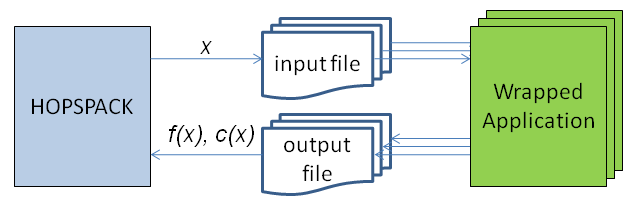
\includegraphics[width=4.0in]{EvalDiagramClipped.png}
    \vspace{-5mm}
  \caption{HOPSPACK communication with an application.}
  \label{fig:callforeval}
  \end{center}
\end{figure}

Figure~\ref{fig:callforeval} shows the flow of data from HOPSPACK to an
application.  Specific variable values at a trial point $x$ are written
to an input file, and the evaluated objective $f(x)$ plus any
nonlinear constraints $c(x)$ are returned via an output file.
%
The figure shows multiple instances of the application running in parallel.
Each instance has its own input and output files, and must run independent
from other application instances.
Figures~\ref{fig:evalMPI} (MPI) and \ref{fig:evalMT} (MT) show examples of how
the applications and HOPSPACK might be distributed across processors and threads.
HOPSPACK helps maintain independence of parallel application instances
by defining a unique ``tag number'' for each evaluation point.  The tag is
used to form unique input and output file names and is made available to
the application instance.  Input and output file names are generated by
HOPSPACK as the concatenation of a string
defined by parameter {\tt Input Prefix} (\PGREF{param:EV-inprefix})
or {\tt Output Prefix} (\PGREF{param:EV-outprefix}), the tag number, and
the evaluation type (discussed below).
The unique tag number allows all files to coexist in the same directory.
If the application creates temporary files, it should use the tag number
to name the files so there is no conflict between parallel instances.
Tag numbers are generated from a counter that is reset whenever HOPSPACK starts;
hence, tag numbers can be reused when HOPSPACK restarts.
 
Input and output file information depends on the type of evaluation information
desired, which is one of the following:
\vspace{-11pt}
\begin{tabbing}
  xxxxxxxxxx \= xxxxx \= \kill
  \> {\tt F}  \> Evaluate the objective $f(x)$ only (no constraints)  \\
  \> {\tt C}  \> Evaluate nonlinear constraints $c(x)$ only (no objective)  \\
  \> {\tt FC} \> Evaluate $f(x)$ and nonlinear constraints $c(x)$
\end{tabbing}
The default type is {\tt FC} since the GSS solver requires all information
at each trial point.  However, a different solver might separate processing
of the objective and constraints; for example, a solver may want to first
find a completely feasible point before requesting the objective value.

The input file begins with two lines of header information and then the value
of each variable.  The first line contains the evaluation type,
and the second line gives the number of variables.
This is followed by variable values, one per line.
The text below shows an example of an input file generated by HOPSPACK for
a problem with two variables:
\vspace{-11pt}
\begin{verbatim}
    FC
    2
    -1.50000000000000e+00
    3.91875000000000e+00
\end{verbatim}

The output file format is similar, with the objective and constraint values
written as vectors in one file.
Objective values are written first
(assuming the evaluation type is {\tt F} or {\tt FC}), and then any nonlinear
constraints (for type {\tt C} or {\tt FC}).
Objective values are written as a vector to allow applications
with multiple objectives.  Constraints are written as
two vectors of values:  one for equalities and one for inequalities.
In all three cases the format of a vector begins with a header line giving
the number of items, and then a list of values, one per line.
If a function cannot be evaluated, the string ``{\tt DNE}'' should be returned,
indicating a value does not exist at the trial point.
The text below shows an example of an output file for type {\tt FC}.
There is one objective (with $f(x) = 5$), no equality constraints,
and two inequalities.
Nonlinear inequalities follow a ``greater than zero'' convention
(\SECREF{subconfig:DEFINITION}), so this particular point is feasible
with respect to the first inequality and infeasible with respect to the second.
Note that HOPSPACK expects the number of objectives to match the value
of configuration parameter
{\tt Number Objectives} (\PGREF{param:PD-numobjs}), and the number of
constraints to match {\tt Number Nonlinear Eqs} (\PGREF{param:PD-numeqs})
and {\tt Number Nonlinear Ineqs} (\PGREF{param:PD-numineqs}).
\vspace{-11pt}
\begin{verbatim}
    1
    5.00000000000000e+00
    0
    2
    1.25000000000000e+02
    -2.08164062500000e+00
\end{verbatim}

When the application wrapper is called to evaluate a particular trial point,
it is given four command line arguments:  the input file name, output file name,
tag number, and evaluation type.  The last argument is repeated on the
first line of the input file.
The application wrapper must read a HOPSPACK input file and create a new
output file before completing.  The wrapper executable itself should return
zero if successful; any other value indicates to HOPSPACK that the evaluation
failed.
An example written in C is provided in the file
{\sf examples/1-var-bnds-only/var\_bnds\_only.c}.  Examples written in C++
are provided in similar subdirectories, including a problem with nonlinear
constraints in {\sf examples/4-nonlinear-constraints/nonlinear\_constraints.cpp}.
The HOPSPACK source code that calls the application is located in
{\sf src/src-evaluator/HOPSPACK\_SystemCall.cpp}.

The application wrapper can return a short error message that will be
reported in HOPSPACK output and passed to solvers.  The point will be
marked as unevaluated, causing it to be ignored by most solvers.
The error message can be a useful mechanism for reporting types of evaluation
failures, instead of simply failing.
If the {\tt Display} parameter from the ``Mediator'' sublist is set to 3
or higher, then the Mediator will print a summary list at the end of execution
showing all evaluation messages that were received.
To send an error message the wrapper executable should return zero
(as though it succeeded), and the message should be on the first line of
the output file instead of the number of objectives.  Everything after the
message will be ignored.
HOPSPACK will attach the message to the point and notify all solvers that
the point could not be evaluated.


%%%%%%%%%%%%%%%%%%%%
\subsection{Linking Evaluation Code}
\label{subcalleval:inlineeval}

The default HOPSPACK mechanism described in \SECREF{subcalleval:systemcall}
evaluates functions by calling the application as a separate process.
A user familiar with C++ can instead link HOPSPACK with the application
code and call it directly.  This mechanism eliminates separate application
processes and file-based communications.  Direct calls will therefore run faster,
although the time savings may be negligible compared to function evaluation
times.
Direct calls also allow run time control of the application through
customization of the ``Evaluator'' sublist of configuration parameters.

Calling the application directly requires modification of HOPSPACK source
code, and linking generally requires changing a CMake build file.
An example is provided in the directory {\sf examples/linked-evaluator-example}.
This example contains a custom {\tt ExampleLinkedEvaluator} class
that implements the {\tt HOPSPACK::Evaluator} interface.  The new class
includes methods {\tt evalF()} and {\tt evalFC()} for computing the
objective function and nonlinear constraints of a specific application.
The example shows how to modify the {\tt HOPSPACK::EvaluatorFactory} class
so it supplies instances of {\tt ExampleLinkedEvaluator}.
More information is given in the file
{\sf examples/linked-evaluator-example/README\_linked\_evaluator.txt}.

If the application depends on specific libraries, then their names must be
given to CMake.  See \SECREF{subsec:cmakeaddlib} for details.

An application called directly has the potential to crash HOPSPACK.
Be sure to surround the call with {\tt try/catch} handlers to trap any
application errors.  If an error is found, the custom evaluator should
return {\tt DNE} values for the functions and a short error message that
will be reported in HOPSPACK output.

An application called directly from the multithreaded version of HOPSPACK must
be thread safe.  HOPSPACK may call {\tt evalFC()} simultaneously
from many threads in the same shared memory space.
%TBD mention AMPL ASL?


%%%%%%%%%%%%%%%%%%%%
\subsection{Evaluation Tips}

For best results, applications should use full numerical precision when
passing values.  HOPSPACK writes variable values to the input file
with 15 significant digits, the maximum number of meaningful digits for double
precision on most machines.  The number of digits can be modified with the
configuration parameter {\tt File Precision} (\PGREF{param:EV-prec}).
The application wrapper should write results to the output file using the
most precision possible.

An application with nonlinear constraints might benefit from careful ordering
of calculations in the application wrapper.  For instance, if some constraints
cannot be violated (sometimes called ``hard constraints''), then it may be
best to check this first and not try to compute the objective function at
an infeasible point.
In this case it is appropriate to return {\tt DNE} for any unevaluated functions.
If the objective is well defined but expensive to compute, then it may be
best to skip evaluating at an infeasible point, returning {\tt DNE} for the
objective.  This causes the constraint to appear as an infinite barrier to
solvers, because an objective value of {\tt DNE} is treated as a value of
infinity ($+\infty$ if minimizing, $-\infty$ if maximizing).
An infinite barrier is nonsmooth and could slow convergence, but the overall
time savings might be worthwhile.

Some solvers might not be capable of working with nonlinear constraints.
In this case the evaluation might choose to return {\tt DNE} when a point
is infeasible.  However, this is not recommended if using the default GSS
solver in HOPSPACK.  GSS computes a penalty for infeasible points and can
make use of the extent to which a point violates constraints.
See \SECREF{subgss} for more.

%%%%%%%%%%%%%%%%%%%%%%%%%%%%%%%%%%%%%%%%%%%%%%%%%%%%%%%%%%%%%%%%%%%%%%
\clearpage
\section{Building HOPSPACK}
\label{sec:build}

HOPSPACK is written with the intent of allowing user modifications and
extensions.  All code is written in C++.  HOPSPACK uses the CMake build
system (\href{http://cmake.org/}{http://cmake.org/}) to support compilation on
multiple platforms, including Linux, Windows, and Mac OSX.  This section
describes the process of installing source code, third party libraries,
and building HOPSPACK executables.
\SECREF{sec:extend} provides examples of modifying or extending
the source code.

Several steps are required to build HOPSPACK.  A quick outline is below,
and full details for various platforms follow.
\begin{list}{x}{\setlength{\itemindent}{20pt}
                \setlength{\itemsep}{-4pt}
                \setlength{\labelsep}{10pt}}
  \item[\ref{subinstall:DN}] Download and unpack HOPSPACK source code.
  \item[\ref{subinstall:CM}] Download and install CMake toolset.
  \item[\ref{subinstall:LA}] Obtain or build an LAPACK library (if linear
                             constraints are used).
  \item[\ref{subinstall:SR}] Build and test a ``serial'' (single processor)
                             HOPSPACK executable.
  \item[\ref{subinstall:MT}] Build and test an ``mt'' (multithreaded)
                             HOPSPACK executable.
  \item[\ref{subinstall:MP}] Build and test an ``mpi'' (multiprocessor)
                             HOPSPACK executable.
  \item[\ref{subinstall:ED}] Complete list of build options.
\end{list}


%%%%%%%%%%%%%%%%%%%%
\subsection{Download HOPSPACK Source Code}
\label{subinstall:DN}

Follow the links at
\vspace{-11pt}
\begin{tabbing}
  xxx \= xxxxxxxxx \= \kill
  \> \href{https://software.sandia.gov/trac/hopspack}
          {https://software.sandia.gov/trac/hopspack}
\end{tabbing}
\vspace{-11pt}
to find the download page.  Please register your email address with
accurate and complete information.  We ask for this information as a
courtesy in exchange for our free software.  Having accurate user data allows
us to better ascertain in what way HOPSPACK is used, which may influence
future development.  Your email address will remain strictly confidential
and will not be used unless you request to be on the HOPSPACK Users Mailing List.
Remember the email address you register so you can registration the next time.

Download the source code.  For convenience, it is supplied in both Windows
compressed file form and Unix compressed tar file form.  The contents are
the same.

Save the compressed file to any directory and unzip it.
You should see a directory structure like the following:
\vspace{-11pt}
\begin{tabbing}
  xxxxxxxxx \= xxx \= xxx \= xxxxxxxxxxxxxxxxxx \= \kill
  \> {\sf hopspack-\HOPSVER.x-src}  \\
  \> \> {\sf doc}                   \\
  \> \> {\sf examples}              \\
  \> \> {\sf src}                   \\
  \> \> {\sf test}
\end{tabbing}


%%%%%%%%%%%%%%%%%%%%
\subsection{Download and Install CMake}
\label{subinstall:CM}

CMake is a leading open-source build system that supports multiple operating
systems.  You need to download a CMake binary distribution
(typically, 5-10 Mbytes in size) appropriate for your operating system
and install it.  If HOPSPACK will run on different machines, then install
CMake on each target machine.
The installation creates a CMake tool that will be used to construct
platform-specific build scripts for compiling HOPSPACK source code.

Visit \href{http://cmake.org/}{http://cmake.org/} and find a recent release
of CMake for your target operating system.  The CMake release must be 2.8.8
or later.  At the time this documentation was produced, the CMake distribution
could be found by clicking on {\sf RESOURCES} and then {\sf Download} to reach
\href{http://cmake.org/cmake/resources/software.html}
     {http://cmake.org/cmake/resources/software.html}.
Only the binary distribution is needed (no CMake source code).
For example, {\tt cmake-2.8.12-Linux-i386.tar.gz} was the file name for
an x86 Linux machine, and {\tt cmake-2.8.12-win32-x86.exe}
the file name for a Windows machine (32-bit or 64-bit).

Installation of CMake is very simple, and explained on the CMake download page.
For example, on a Linux machine just unpack the file to any directory
(this procedure does not require root privileges).
It should create a new subdirectory tree with a name like
{\tt cmake-2.8.12-Linux-i386}.
Just add the subdirectory {\tt cmake-2.8.12-Linux-i386/bin} to {\tt PATH}.

On Windows, run the CMake distribution file to start an installation wizard
and follow the directions.  By default, CMake will install at
{\tt C:$\backslash$$\backslash$Program~Files$\backslash$CMake~2.8}
and create a {\sf Start~Menu} entry that invokes the CMake GUI interface.
If you prefer to run the command line version of CMake, then click a wizard
button that adds CMake to {\tt PATH}.


%%%%%%%%%%%%%%%%%%%%
\subsection{Build an LAPACK Library}
\label{subinstall:LA}

A third party LAPACK (Linear Algebra PACKage) library is required for
optimization problems with general linear constraints.  Simple variable bounds
do not require LAPACK.  If your problems do not have general linear constraints,
then skip the rest of this section, but add the command line option
{\tt -Dlapack:BOOL=false} when building HOPSPACK.  The option tells the build to
modify source code so that no calls to LAPACK are made; however, it also prevents
HOPSPACK from solving problems with linear constraints.

Your system may already have LAPACK installed.  For instance, on some Linux
distributions LAPACK is available in the file {\sf /usr/lib/liblapack.a}.
In this case CMake should find it automatically and no further effort is
needed.  Try building the serial executable as described in
\SECREF{subinstall:SR}; the CMake configuration will tell you clearly
whether an LAPACK library was found.

If LAPACK was not found on your system, or you prefer a particular version,
then the library must be installed.  LAPACK libraries are available from
many sources.
One of the most popular versions is from Netlib, freely available at
\href{http://netlib.sandia.gov/}{http://netlib.sandia.gov/}.
Other possibilities are vendor-provided libraries like the Intel MKL or
AMD ACML, and tunable versions such as ATLAS.

LAPACK functions called by HOPSPACK are the following:
\vspace{-11pt}
\begin{tabbing}
  xxxxxxxx \= xxxxxxxxxx \= xxxxxxxxxx \= \kill
  \> {\tt ddot}   \> {\tt dgemm}   \> {\tt dgglse} \\
  \> {\tt dgelqf} \> {\tt dgemv}                   \\
  \> {\tt dgelss} \> {\tt dgesvd}
\end{tabbing}
\vspace{-11pt}
Make sure the library contains these functions and their dependents, or there
will be unresolved symbols when linking the final HOPSPACK executable.
CMake will test for the presence of these functions when it
configures HOPSPACK, and will halt with a warning message if it detects
a problem.

\bigskip
\noindent{\bf Linux example of building Netlib.}
This example shows a particular case of building a Netlib library that is
compatible with CMake.  Netlib produces two library files, one for BLAS
functions such as {\tt ddot} and one for LAPACK functions such as {\tt dgglse}.
The Netlib libraries
are created using a Fortran compiler, so the HOPSPACK C++ executables
must include a Fortran-to-C library (the CMake build process will try to do
this automatically).
Please note this is just one possible example and your build procedure
may differ.
\begin{tabbing}
  xxx \= xxx \= xxx \= \kill
  \> - Download {\sf lapack-3.4.0.tgz} from
       \href{http://netlib.sandia.gov/lapack/}
            {http://netlib.sandia.gov/lapack}  \\
  \> - Unpack the distribution (this example assumes the directory {\tt /tmp}
       is used) \\
  \> - Create a build directory and {\tt cd} to it;
       here, assume {\tt /tmp/bld} is used  \\
  \> \> {\tt > cd /tmp/bld}  \\
  \> \> {\tt > cmake ../lapack-3.4.0}  \\
  \> \> {\tt > make}  \\
  \> \> This should create a subdirectory {\sf lib} containing
        {\sf libblas.a} and {\sf liblapack.a}  \\
  \> - Add these options to the CMake command line  \\
  \>   \; (note the semicolon separator, a CMake requirement):  \\
  \> \> {\tt -DLAPACK\_LIBS="\$LH/liblapack.a;\$LH/libblas.a"}  \\
  \> \> (where {\tt \$LH} is the LAPACK home {\tt /tmp/lapack-3.4.0/lib})  \\
  \> - If CMake has trouble finding the Fortran-to-C library, try adding:  \\
  \> \> {\tt -DLAPACK\_ADD\_LIBS=gfortran}
\end{tabbing}
%-----OLD METHOD:
%This example shows a particular case of building a Netlib version using the GNU
%compilers.  Netlib produces two library files, one for BLAS functions such
%as {\tt ddot} and one for LAPACK functions such as {\tt dgglse}.
%The Netlib libraries
%are created using a Fortran compiler, so the HOPSPACK C++ executables
%must include a Fortran-to-C library (the CMake build process will try to do
%this automatically).
%The example also shows how to edit the HOPSPACK CMake configuration file to
%find the libraries if they are produced in a nonstandard location.
%Please note this is just one possible example and your build procedure
%may differ.
%\begin{tabbing}
%  xxx \= xxx \= xxx \= \kill
%  \> - Download {\sf lapack-3.1.1.tgz} from
%       \href{http://netlib.sandia.gov/lapack/}
%            {http://netlib.sandia.gov/lapack}  \\
%  \> - Unpack the distribution (this example assumes the directory {\tt /tmp}
%       is used) \\
%  \> - Consult {\sf README} and {\sf INSTALL/lawn81.pdf} for Netlib
%       instructions.  \\
%
%  \> - For a Linux RHEL 4 machine build a minimal LAPACK as follows:  \\
%  \> \> {\tt > cp make.inc.example make.inc}  \\
%  \> \> Edit {\sf Makefile}:  \\
%  \> \> \> Change comments to enable building {\tt blaslib} and
%           {\tt lapacklib}\\
%  \> \> \> Change ``{\tt \$(MAKE)}'' to ``{\tt \$(MAKE) double}''
%         to avoid unnecessary objects  \\
%  \> \> {\tt > make lib} $\;$ (should produce files {\sf blas\_LINUX.a}
%                               and {\sf lapack\_LINUX.a})  \\
%  \> \> Netlib libraries must be renamed to conform with Linux convention: \\
%  \> \> {\tt > mv blas\_LINUX.a libblas\_LINUX.a}  \\
%  \> \> {\tt > mv lapack\_LINUX.a liblapack\_LINUX.a}  \\
%
%  \> - Either add these options to the CMake command line:  \\
%  \> \> {\tt -DLAPACK\_LIBS="\$LH/liblapack\_LINUX.a;\$LH/libblas\_LINUX.a"}  \\
%  \> \> (where {\tt \$LH} is the LAPACK home {\tt /tmp/lapack-3.1.1})  \\
%  \> - Or edit {\sf ConfigureLapack.cmake} in the HOPSPACK directory:  \\
%  \> \> Find the section beginning with the message
%        ``Linear constraints allowed''  \\
%  \> \> Comment out option 1 and uncomment the lines for option 3  \\
%  \> \> Change the path in option 3 to the location of your libraries  \\
%  \> \> (Use option 2 if your libraries are in a standard location)  \\
%  \> - If CMake has trouble finding the Fortran-to-C library, try adding:  \\
%  \> \> {\tt -DLAPACK\_ADD\_LIBS="gfortran"}
%\end{tabbing}

\medskip
\noindent{\bf Windows example of using Netlib with MSVC.}
This example uses a CMake-compatible version of the Netlib source code that
is compiled with the Microsoft Visual C++ compiler (MSVC++).
The example describes how to build from the command line; the CLAPACK web site
describes how to build using Visual Studio.
The command line procedure follows:
\begin{tabbing}
  xxx \= xxx \= xxx \= \kill
  \> - Download {\sf clapack-3.2.1-CMAKE.tgz} from
       \href{http://icl.cs.utk.edu/lapack-for-windows/clapack/}
            {http://icl.cs.utk.edu/lapack-for-windows/clapack}  \\
  \> - Unzip the distribution in any directory;
       here, assume {\tt c:$\backslash$temp} is used  \\
  \> - Create a build directory and {\tt cd} to it;
       here, assume {\tt c:$\backslash$temp$\backslash$bld} is used  \\
  \> \> {\tt > cd c:$\backslash$temp$\backslash$bld}  \\
  \> \> {\tt > cmake -G "NMake Makefiles" .. -DCMAKE\_BUILD\_TYPE=Release}  \\
  \> \> \> {\tt -DCMAKE\_INSTALL\_PREFIX="c:$\backslash$$\backslash$temp$\backslash$$\backslash$netlibinstall"}  \\
  \> \> {\tt > nmake}  \\
  \> \> {\tt > nmake install}  \\
  \> - Directory {\sf c:$\backslash$temp$\backslash$netlibinstall$\backslash$lib}
       should be created, with three {\sf .lib} files inside \\
  \> - Define an environment variable  \\
  \> \> {\tt > set LP=c:$\backslash$temp$\backslash$netlibinstall$\backslash$lib}  \\
  \> - Add these options to the CMake command line:  \\
  \> \> \> {\tt -DLAPACK\_LIBS="\%LP\%$\backslash$blas.lib;\%LP\%$\backslash$lapack.lib"}  \\
  \> \> \> {\tt -DLAPACK\_ADD\_LIBS=\%LP\%$\backslash$libf2c.lib}
\end{tabbing}

\medskip
\noindent{\bf Linux example of using Intel MKL.}
The Intel MKL contains routines for LAPACK and many other math functions that
are specially tuned for Intel microprocessors.  You could use the MKL builder
tool to create a single library containing just the LAPACK routines needed
by HOPSPACK.  In that case, pass the library to CMake using the command line
option {\tt -DLAPACK\_LIBS}.
Another technique is to provide all the appropriate MKL libraries to CMake and
let the linker find what it needs.  Assuming {\tt \$MKL\_LIB} is the directory
where MKL libraries are stored, the CMake command line options are
(for MKL version 10.3.7):

\hspace{0.2in}
{\tt -DLAPACK\_LIBS=\$MKL\_LIB/libmkl\_rt.so}

\noindent or for MKL version 9.0:

\hspace{0.2in}
{\tt -DLAPACK\_LIBS="\$MKL\_LIB/libmkl\_lapack.a;\$MKL\_LIB/libmkl\_ia32.a"}

\vspace{-11pt}
\hspace{0.2in}
{\tt -DLAPACK\_ADD\_LIBS=\$MKL\_LIB/libguide.so}


%%%%%%%%%%%%%%%%%%%%
\subsection{Build and Test the ``serial'' HOPSPACK Executable}
\label{subinstall:SR}

The CMake tool constructs platform-specific build scripts for compiling and
linking executables.  We recommend making an ``out of source'' build, instead of
building the object and executable files in the source directories.  This is
easy to do with CMake and allows the existence of multiple builds without
conflict; for instance, a serial and MPI build.

To create an out of source build, make a clean directory,
change to it, and run CMake from this directory.  CMake allows the build
directories to be anywhere, but in the remainder of this section we assume a
clean directory is created at the same level as {\sf hopspack-\HOPSVER.x-src}.
After building and installing at the default location,
the directory structure will look like the following (not all files are shown):
\vspace{-11pt}
\begin{tabbing}
  xxxxxxxxx \= xxx \= xxx \= xxx \= xxxxxxxxxxxxxxxxxx \= \kill
  \> {\sf hopspack-\HOPSVER.x-src}  \\
  \> \> {\sf doc}                      \> \> \> (provided)    \\
  \> \> {\sf examples}                 \> \> \> (provided)    \\
  \> \> {\sf src}                      \> \> \> (provided)    \\
  \> \> {\sf test}                     \> \> \> (provided)    \\
  \> {\sf build\_serial}            \> \> \> \> (create this and build in it)  \\
  \> \> {\sf installed\_HOPSPACK}      \> \> \> (built by CMake install)  \\
  \> \> \> {\tt HOPSPACK\_main\_serial}   \> \> (built by CMake install)  \\
  \> \> \> {\sf examples}                 \> \> (built by CMake install)  \\
  \> \> \> \> {\sf 1-var-bnds-only}          \> (built by CMake install)  \\
  \> \> \> \> {\sf ...}                      \> (built by CMake install)  \\
  \> \> \> {\sf test}                     \> \> (built by CMake install)
\end{tabbing}

The examples below show how to run CMake on various platforms.
For information on linking with an LAPACK library, see \SECREF{subinstall:LA}.
LAPACK linking can be troublesome on some machines; if necessary, try linking
without it by adding the CMake option {\tt -Dlapack:BOOL=false} (however,
this will limit HOPSPACK from solving problems with linear constraints).
For trouble-shooting or customizing CMake, see \SECREF{sec:cmake}.


\bigskip
\noindent {\bf Linux (build serial HOPSPACK).}
Start at the HOPSPACK parent directory and run the following commands:
\vspace{-11pt}
\begin{tabbing}
  xxx \= \kill
  \> {\tt > mkdir build\_serial} \\
  \> {\tt > cd build\_serial} \\
  \> {\tt > cmake ../hopspack-\HOPSVER.x-src} \\
  \> {\tt -- The CXX compiler identification is GNU} \\
  \> {\tt -- ...} \\
  \> {\tt -- Build files have been written to: ...} \\
  \> {\tt > make} (or {\tt gmake}) \\
  \> {\tt > make test} \\
  \> {\tt > make install}
\end{tabbing}
\vspace{-11pt}
The execution of {\tt cmake} displays several lines of informational output,
only a few of which are shown above.  Its behavior is roughly similar to a
Unix ``autoconf'' or ``config'' tool.
It produces a subdirectory structure similar to that of
{\sf hopspack-\HOPSVER.x-src},
with {\tt Makefile} files that work with the chosen compiler.  Running
{\tt make} in the last step produces the HOPSPACK executable, test executables,
and optimization evaluators in {\sf examples}.
Running {\tt make test} invokes CTest (a CMake utility) to run any automated
tests that come with HOPSPACK.  They should all pass.

Now change to the {\sf installed\_HOPSPACK/examples} directory.
There should be a number of
subdirectories named {\sf 1-var-bnds-only, 2-linear-constraints}, etc.,
and a {\sf README.txt} file.  Each subdirectory contains HOPSPACK
configuration parameters and a small executable that evaluates optimization
objectives and constraints at a given point.
Run the first example:
\vspace{-11pt}
\begin{tabbing}
  xxx \= \kill
  \> {\tt > cd examples/1-var-bnds-only} \\
  \> {\tt > ../../HOPSPACK\_main\_serial example1\_params.txt}
\end{tabbing}
\vspace{-11pt}
As explained in the {\sf README.txt} file, this solves a simple two-dimensional
minimization problem with bound constraints.  Check the solution against
the value listed in {\sf README.txt}.
Try {\sf 2-linear-constraints} if your configuration includes an LAPACK file
for problems with linear constraints.

A common problem on Linux machines is failure of example evaluations because
the current directory is not in the {\tt PATH} environment variable.
An error message

\hspace{0.2in}
{\tt ERROR: Call failed: `var\_bnds\_only ...' <SystemCall>}

\noindent
means the Evaluator in HOPSPACK could not run the example executable.
An easy fix is to add the current directory to the PATH environment variable:
\vspace{-11pt}
\begin{tabbing}
  xxx \= \kill
  \> {\tt > export PATH=\$PATH:.}
\end{tabbing}
\vspace{-11pt}
Alternatively, edit {\sf example1\_params.txt} and change the parameter
defining the executable to be

\hspace{0.2in}
{\tt  "Executable Name" string "./var\_bnds\_only"}


\bigskip
\noindent {\bf Mac OSX (build serial HOPSPACK).}
This section assumes a recent version of XCode is installed on the Mac,
providing a g++ compiler and LAPACK libraries.  Usually, libraries
appear as the files {\sf /usr/lib/libblas.dylib}
and {\sf /usr/lib/liblapack.dylib}.
% True for XCode 3.1.2 on Mac OSX 10.5.8, XCode 3.2 on Mac OSX 10.6.8

Open a Mac Terminal Window and follow the same procedure as the Linux build
example described immediately above.  The only difference is that the additional
LAPACK library name must be passed to CMake during configuration.  Do this
with the option {\tt -DLAPACK\_ADD\_LIBS}:
\vspace{-11pt}
\begin{tabbing}
  xxx \= \kill
  \> {\tt > mkdir build\_serial} \\
  \> {\tt > cd build\_serial} \\
  \> {\tt > cmake ../hopspack-\HOPSVER.x-src
                  -DLAPACK\_ADD\_LIBS=/usr/lib/libblas.dylib} \\
  \> {\tt -- ...} \\
  \> {\tt > make} (or {\tt gnumake}) \\
  \> {\tt > make test} \\
  \> {\tt > make install}
\end{tabbing}
\vspace{-11pt}
This will build the executable program {\tt HOPSPACK\_main\_serial}.

Now change to the {\sf installed\_HOPSPACK/examples} directory.
There should be a number of
subdirectories named {\sf 1-var-bnds-only, 2-linear-constraints}, etc.,
and a {\sf README.txt} file.  Each subdirectory contains HOPSPACK
configuration parameters and a small executable that evaluates optimization
objectives and constraints at a given point.
Run the first example:
\vspace{-11pt}
\begin{tabbing}
  xxx \= \kill
  \> {\tt > cd examples/1-var-bnds-only} \\
  \> {\tt > ../../HOPSPACK\_main\_serial example1\_params.txt}
\end{tabbing}
\vspace{-11pt}
As explained in the {\sf README.txt} file, this solves a simple two-dimensional
minimization problem with bound constraints.  Check the solution against
the value listed in {\sf README.txt}.

A common problem is failure of example evaluations because
the current directory is not in the {\tt PATH} environment variable.
See the Linux build example above for more information.


\bigskip
\noindent {\bf Windows using Visual Studio (build serial HOPSPACK).}
CMake can generate a Microsoft Visual Studio project for the HOPSPACK
source code, which can then be compiled and tested using Visual Studio.
This example assumes the free {\it Visual Studio C++ 2010 Express Edition}
is installed.
An example in the next section describes how CMake can produce a set of
{\tt Makefile} files that work with the command line {\tt nmake} tool in the
Express Edition.

CMake can execute in a GUI or from the command line.  This example uses
a Windows DOS-like command line console such as the one below.

\begin{center}
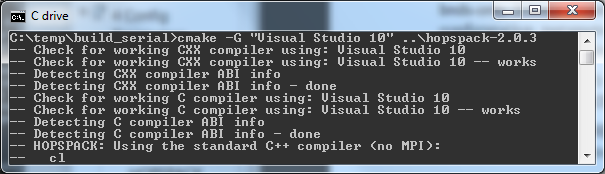
\includegraphics[width=5.5in]{winconsole_cmake_msvc.png}
\end{center}

First, make sure environment variables are configured for the Microsoft compiler.
If installed in its default location, this is accomplished (for version 10.0)
by running:
\vspace{-11pt}
\begin{tabbing}
  xxx \= \kill
  \> {\tt > c:$\backslash$Program Files$\backslash$Microsoft Visual Studio 10.0$\backslash$VC$\backslash$bin$\backslash$vcvars32.bat}
\end{tabbing}

Start at the directory where the HOPSPACK parent directory exists and
run the following commands:
\vspace{-11pt}
\begin{tabbing}
  xxx \= \kill
  \> {\tt > mkdir build\_serial} \\
  \> {\tt > cd build\_serial} \\
  \> {\tt > cmake -G "Visual Studio 10" ..$\backslash$hopspack-\HOPSVER.x-src} \\
  \> {\tt -- Check for working CXX compiler using: Visual Studio 10} \\
  \> {\tt -- ...} \\
  \> {\tt -- Build files have been written to: ...}
\end{tabbing}
\vspace{-11pt}
The execution of {\tt cmake} displays several lines of informational output,
only a few of which are shown above.
It produces a subdirectory structure similar to that of
{\sf hopspack-\HOPSVER.x-src},
and a file {\sf ALL\_BUILDS.vcxproj} with the main Visual Studio project.

Start Visual Studio and open the file {\sf ALL\_BUILDS.vcxproj}.  It contains
projects for all the libraries and executables built by HOPSPACK.
If you build {\tt ALL\_BUILDS} then Visual Studio will compile and link
everything, including the serial HOPSPACK executable, examples, and tests.
A successful build is shown in the screen shot below.

\begin{center}
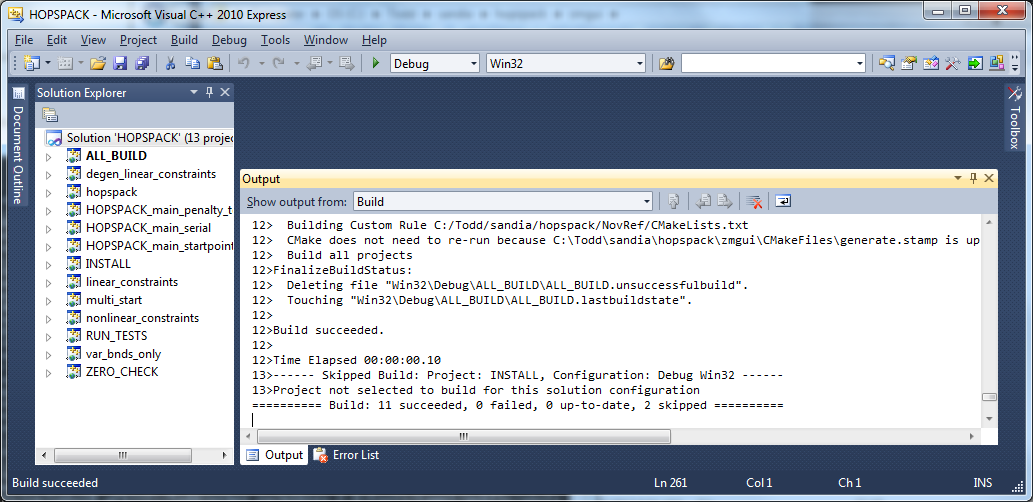
\includegraphics[width=5.0in]{winmsvc_build.png}
\end{center}

You must return to a command line console to run HOPSPACK.
The main executable should be under the {\sf src} directory:
{\sf build\_serial$\backslash$src$\backslash$src-main$\backslash$Debug$\backslash$HOPSPACK\_main\_serial.exe} in this example.  You can move the file to a
more convenient location if desired.

Now open a command line console and change to the {\sf examples} directory.
There should be a number of
subdirectories named {\sf 1-var-bnds-only, 2-linear-constraints}, etc.,
and a {\sf README.txt} file.  Each subdirectory contains HOPSPACK
configuration parameters and a small executable that evaluates optimization
objectives and constraints at a given point.
You may have to edit the parameters file in each example and tell it where
the optimization executable is located.
Run the first example:
\vspace{-11pt}
\begin{tabbing}
  xxx \= xxxxx \= \kill
  \> {\tt > cd examples$\backslash$1-bnd-vars-only} \\
  \> Edit {\sf example1\_params.txt} and change the ``Executable Name'' parameter
     to be \\
  \> \> {\tt "Executable Name" string "Debug$\backslash$var\_bnds\_only.exe"} \\
  \> {\tt > ..$\backslash$..$\backslash$src$\backslash$src-main$\backslash$Debug$\backslash$HOPSPACK\_main\_serial.exe example1\_params.txt}
\end{tabbing}
\vspace{-11pt}
As explained in the {\sf README.txt} file, this solves a simple two-dimensional
minimization problem with bound constraints.  Check the solution against
the value listed in {\sf README.txt}.
Try {\sf 2-linear-constraints} if your configuration includes an LAPACK file
for problems with linear constraints.


\bigskip
\noindent {\bf Windows using NMake (build serial HOPSPACK).}
CMake can generate a set of {\tt Makefile} files that work with the
Visual Studio command line {\tt nmake} tool.  The {\tt nmake} facility is
provided with the full Microsoft Visual Studio product or the free
Visual Studio Express Edition (available from Microsoft).

This section assumes {\it Visual C++ 2010 Express Edition} with the
version 10.0 compiler is installed.  All commands are run from
a Windows DOS-like command line console such as the one below.

\begin{center}
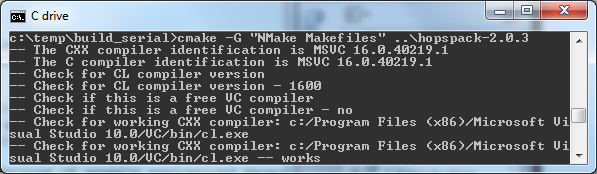
\includegraphics[width=5.5in]{winconsole_cmake.png}
\end{center}

First, make sure environment variables are configured for the Microsoft compiler.
If installed in its default location, this is accomplished (for version 10.0)
by running:
\vspace{-11pt}
\begin{tabbing}
  xxx \= \kill
  \> {\tt > c:$\backslash$Program Files$\backslash$Microsoft Visual Studio 10.0$\backslash$VC$\backslash$bin$\backslash$vcvars32.bat}
\end{tabbing}

Start at the directory where the HOPSPACK parent directory exists and
run the following commands:
\vspace{-11pt}
\begin{tabbing}
  xxx \= \kill
  \> {\tt > mkdir build\_serial} \\
  \> {\tt > cd build\_serial} \\
  \> {\tt > cmake -G "NMake Makefiles"
            ..$\backslash$hopspack-\HOPSVER.x-src} \\
  \> {\tt -- The CXX compiler identification is MSVC ...} \\
  \> {\tt -- ...} \\
  \> {\tt -- Build files have been written to: ...} \\
  \> {\tt > nmake} \\
  \> {\tt > nmake install}
\end{tabbing}
\vspace{-11pt}
The execution of {\tt cmake} displays several lines of informational output,
only a few of which are shown above.
It produces a subdirectory structure similar to that of
{\sf hopspack-\HOPSVER.x-src},
with {\tt Makefile} files that work with the chosen compiler.  Running
{\tt nmake} from the command line produces the HOPSPACK executable, test
executables, and optimization evaluators in {\sf examples}.
Running {\tt nmake install} copies appropriate files into a new subdirectory
named {\sf installed\_HOPSPACK}.

Now change to the {\sf installed\_HOPSPACK$\backslash$examples} directory.
There should be a number of
subdirectories named {\sf 1-var-bnds-only, 2-linear-constraints}, etc.,
and a {\sf README.txt} file.  Each subdirectory contains HOPSPACK
configuration parameters and a small executable that evaluates optimization
objectives and constraints at a given point.
Run the first example:
\vspace{-11pt}
\begin{tabbing}
  xxx \= \kill
  \> {\tt > cd examples$\backslash$1-bnd-vars-only} \\
  \> {\tt > ..$\backslash$..$\backslash$HOPSPACK\_main\_serial.exe example1\_params.txt}
\end{tabbing}
\vspace{-11pt}
As explained in the {\sf README.txt} file, this solves a simple two-dimensional
minimization problem with bound constraints.  Check the solution against
the value listed in {\sf README.txt}.
Try {\sf 2-linear-constraints} if your configuration includes an LAPACK file
for problems with linear constraints.


%%%%%%%%%%%%%%%%%%%%
\subsection{Build and Test an ``mt'' HOPSPACK Executable}
\label{subinstall:MT}

This section assumes you are making an ``out of source'' multithreaded build
in a separate directory from the serial build of Section~\ref{subinstall:SR}.
After building and installing at the default location,
the directory structure will look like the following (not all files are shown):
\vspace{-11pt}
\begin{tabbing}
  xxxxxxxxx \= xxx \= xxx \= xxx \= xxxxxxxxxxxxxxxxxx \= \kill
  \> {\sf hopspack-\HOPSVER.x-src}  \\
  \> \> {\sf doc}                      \> \> \> (provided)    \\
  \> \> {\sf examples}                 \> \> \> (provided)    \\
  \> \> {\sf src}                      \> \> \> (provided)    \\
  \> \> {\sf test}                     \> \> \> (provided)    \\
  \> {\sf build\_mt}                \> \> \> \> (create this and build in it)  \\
  \> \> {\sf installed\_HOPSPACK}      \> \> \> (built by CMake install)  \\
  \> \> \> {\tt HOPSPACK\_main\_threaded} \> \> (built by CMake install)  \\
  \> \> \> {\sf examples}                 \> \> (built by CMake install)  \\
  \> \> \> \> {\sf 1-var-bnds-only}          \> (built by CMake install)  \\
  \> \> \> \> {\sf ...}                      \> (built by CMake install)  \\
  \> \> \> {\sf test}                     \> \> (built by CMake install)
\end{tabbing}

The build procedure is almost identical to that of Section~\ref{subinstall:SR}.
An extra option is passed to CMake that instructs it to find
multithreading libraries and compile additional thread-based source files.
You can create separate serial and MPI versions of HOPSPACK if for some
reason multithreading libraries are not available on your machine.

All the examples in Section~\ref{subinstall:SR} begin with three instructions:
create a new directory, change to it, and run CMake.
To build the multithreaded version, similar instructions are typed
in at the command line, but with the option {\tt -Dmt=yes}:
\vspace{-11pt}
\begin{tabbing}
  xxx \= \kill
  \> {\tt > mkdir build\_mt} \\
  \> {\tt > cd build\_mt} \\
  \> {\tt > cmake ../hopspack-\HOPSVER.x-src -Dmt=yes}
\end{tabbing}

From this point, the build procedure is identical to Section~\ref{subinstall:SR}.
Note that CMake accepts any of the option values {\tt -Dmt=yes}, {\tt -Dmt=true},
or {\tt -Dmt=on}.

Assuming the build completed successfully, change to the {\sf examples}
directory.  There should be a number of subdirectories named
{\sf 1-var-bnds-only, 2-linear-constraints}, etc., and a {\sf README.txt} file.
Each subdirectory contains HOPSPACK configuration parameters and a small
executable that evaluates optimization objectives and constraints at a given
point.
Run the first example:
\vspace{-11pt}
\begin{tabbing}
  xxx \= \kill
  \> {\tt > cd examples/1-var-bnds-only} \\
  \> {\tt > ../../HOPSPACK\_main\_threaded example1\_params.txt}
\end{tabbing}
\vspace{-11pt}
As explained in the {\sf README.txt} file, this solves a simple two-dimensional
minimization problem with bound constraints.  Check the solution against
the value listed in {\sf README.txt}.
The {\tt Number Threads} parameter in the ``Mediator'' sublist
(\PGREF{param:MD-numthreads}) determines how many threads are created.
Try increasing the number of threads and observe that more ``Eval workers''
are used.

If the {\tt Display} parameter in the ``Mediator'' sublist
(\PGREF{param:MD-display}) is 3 or larger,
then a timing report for each evaluation worker will be printed after
HOPSPACK completes.  The value displayed is the cumulative wall clock time that
the Executor believes a worker is busy.  This should be nearly the same as the
time consumed by evaluations on a worker, assuming the machine has sufficient
processors to handle each worker thread.  However, if workers do not have
available processors when they are assigned work by the Executor, then the
displayed time will be longer than actual evaluation time.

Source files used in the multithreaded version are identical to those used
in the serial version except for the main routine
({\sf HOPSPACK\_main\_threaded.cpp} versus {\sf HOPSPACK\_main\_serial.cpp}),
and the executor
({\sf HOPSPACK\_ExecutorMultiThreaded.cpp} versus
{\sf HOPSPACK\_ExecutorSerial.cpp}).
In addition, the ``shared'' library includes classes that wrap native
threading functions ({\sf src/src-shared/HOPSPACK\_Thread*}).


%%%%%%%%%%%%%%%%%%%%
\subsection{Build and Test an ``mpi'' HOPSPACK Executable}
\label{subinstall:MP}

This section assumes you have read about building a serial executable in
Section~\ref{subinstall:SR}.  Differences for building with MPI are discussed
here, but refer to Section~\ref{subinstall:SR} for more details about building
with CMake.

This section assumes you are making an ``out of source'' MPI build in a separate
directory from the serial build of Section~\ref{subinstall:SR}.
After building and installing at the default location,
the directory structure will look like the following (not all files are shown):
\vspace{-11pt}
\begin{tabbing}
  xxxxxxxxx \= xxx \= xxx \= xxx \= xxxxxxxxxxxxxxxxxx \= \kill
  \> {\sf hopspack-\HOPSVER.x-src}  \\
  \> \> {\sf doc}                      \> \> \> (provided)    \\
  \> \> {\sf examples}                 \> \> \> (provided)    \\
  \> \> {\sf src}                      \> \> \> (provided)    \\
  \> \> {\sf test}                     \> \> \> (provided)    \\
  \> {\sf build\_mpi}               \> \> \> \> (create this and build in it)  \\
  \> \> {\sf installed\_HOPSPACK}      \> \> \> (built by CMake install)  \\
  \> \> \> {\tt HOPSPACK\_main\_mpi}      \> \> (built by CMake install)  \\
  \> \> \> {\sf examples}                 \> \> (built by CMake install)  \\
  \> \> \> \> {\sf 1-var-bnds-only}          \> (built by CMake install)  \\
  \> \> \> \> {\sf ...}                      \> (built by CMake install)  \\
  \> \> \> {\sf test}                     \> \> (built by CMake install)
\end{tabbing}

The build procedure is almost identical to that of Section~\ref{subinstall:SR}.
An extra option is passed to CMake that instructs it to find
MPI libraries and compile with an MPI-aware compiler.
You can create separate serial and multithreaded versions of HOPSPACK if for
some reason MPI fails to build on your machine.

All the examples in Section~\ref{subinstall:SR} begin with three instructions:
create a new directory, change to it, and run CMake.
To build the MPI version, similar instructions are typed
in at the command line, but with the option {\tt -Dmpi=yes}:
\vspace{-11pt}
\begin{tabbing}
  xxx \= \kill
  \> {\tt > mkdir build\_mpi} \\
  \> {\tt > cd build\_mpi} \\
  \> {\tt > cmake ../hopspack-\HOPSVER.x-src -Dmpi=yes}
\end{tabbing}
\vspace{-11pt}
If CMake has trouble finding your MPI-aware compiler, try specifying
it as a command line parameter; for example:
\vspace{-11pt}
\begin{tabbing}
  xxx \= \kill
  \> {\tt > cmake ../hopspack-\HOPSVER.x-src -Dmpi=yes
            -DMPI\_COMPILER=/tmp/mpich-1.2.7p1/bin/mpicxx}
\end{tabbing}
\vspace{-11pt}
If this fails, consider modifying {\sf ConfigureMPI.cmake}.  This file contains
some comments about the procedure CMake uses to find and configure MPI.

From this point, the build procedure is identical to Section~\ref{subinstall:SR}.
Note that CMake accepts any of the option values {\tt -Dmpi=yes},
{\tt -Dmpi=true}, or {\tt -Dmpi=on}.

Assuming the build completed successfully, change to the {\sf examples}
directory.  There should be a number of subdirectories named
{\sf 1-var-bnds-only, 2-linear-constraints}, etc., and a {\sf README.txt} file.
Each subdirectory contains HOPSPACK configuration parameters and a small
executable that evaluates optimization objectives and constraints at a given
point.
Run the first example:
\vspace{-11pt}
\begin{tabbing}
  xxx \= \kill
  \> {\tt > cd examples/1-var-bnds-only} \\
  \> {\tt > mpirun -np 2 ../../HOPSPACK\_main\_mpi example1\_params.txt}
\end{tabbing}
\vspace{-11pt}
As explained in the {\sf README.txt} file, this solves a simple two-dimensional
minimization problem with bound constraints.  Check the solution against
the value listed in {\sf README.txt}.
The {\tt Number Processors} parameter in the ``Mediator'' sublist
(\PGREF{param:MD-numproc}) determines how many processors are used.
Try increasing the number (along with the argument for {\tt -np})
and observe that more ``Eval workers'' are used.

If the {\tt Display} parameter in the ``Mediator'' sublist
(\PGREF{param:MD-display}) is 3 or larger,
then a timing report for each evaluation worker will be printed after
HOPSPACK completes.  The value displayed is the cumulative wall clock time that
the Executor believes a worker is busy.  Time is measured by the Executor on
the main MPI node, not the worker.  The Executor measures from the moment
an MPI message is sent to a worker to the moment an MPI reply is received.

Source files used in the MPI version are identical to those used
in the serial version except for the main routine
({\sf HOPSPACK\_main\_mpi.cpp} versus {\sf HOPSPACK\_main\_serial.cpp}),
and the executor
({\sf HOPSPACK\_ExecutorMpi.cpp} versus
{\sf HOPSPACK\_ExecutorSerial.cpp}).
In addition, the ``shared'' library includes a class that wraps MPI
functions ({\sf src/src-shared/HOPSPACK\_GenProcComm}).


%%%%%%%%%%%%%%%%%%%%
\subsection{List of Build Options for HOPSPACK}
\label{subinstall:ED}

The list below describes HOPSPACK build options available at the CMake
command line.  All options should be preceded with ``{\tt -D}''.
If the option is a Boolean flag, then the option should be followed
with ``{\tt =true}'' or ``{\tt =false}'' with no intervening spaces.

\begin{itemize}
  \item {\tt mt} $\;$
      Boolean option that instructs CMake to build a parallel HOPSPACK with
      multithreading.  See Section~\ref{subinstall:MT}.
  \item {\tt mpi} $\;$
      Boolean option that instructs CMake to build a parallel HOPSPACK for MPI.
      See Section~\ref{subinstall:MP}.
  \item {\tt lapack} $\;$
      Boolean option that instructs CMake to link with LAPACK for optimization
      problems with linear constraints.  The option is true by default.
      See Section~\ref{subinstall:LA}.
  \item {\tt LAPACK\_LIBS} $\;$
      Set the value to the (nonstandard) location of LAPACK libraries.
      See Section~\ref{subinstall:LA}.
  \item {\tt LAPACK\_ADD\_LIBS} $\;$
      Set the value to the location of additional libraries needed to
      satisfy LAPACK link dependencies.
      See Section~\ref{subinstall:LA}.
  \item {\tt HAVE\_CDDLIB} $\;$
      Boolean option that instructs CMake to include CDDLIB code for
      optimization problems with degenerate linear constraints.  The option
      is true by default.  If CDDLIB is disabled, then
      {\sf examples/3-degen-linear-constraints} will fail.
      Including CDDLIB changes the open source license status of HOPSPACK;
      see Section~\ref{subintro:licenses} for details.
  \item {\tt CMAKE\_INSTALL\_PREFIX} $\;$
      Set the value to the name of a directory where CMake should install
      final executables and examples.  The default is a directory named
      {\sf installed\_HOPSPACK} under the build directory where CMake
      is invoked.
  \item {\tt HOPSPACK\_DEBUG} $\;$
      Boolean option that instructs the native compiler to create
      a debuggable version of HOPSPACK executables.
\end{itemize}

%%%%%%%%%%%%%%%%%%%%%%%%%%%%%%%%%%%%%%%%%%%%%%%%%%%%%%%%%%%%%%%%%%%%%%
\clearpage
\section{Extending HOPSPACK}
\label{sec:extend}

The HOPSPACK framework is written with the intention that users will extend it
to suit their own needs.  Software is written in C++ and follows object
oriented design practices.  The code compiles on major platforms using the
CMake build tool (see \SECREF{sec:cmake}).

Comments throughout the code conform
to Doxygen standards (\href{http://www.doxygen.org/}{http://www.doxygen.org/})
for automated source code documentation.  HTML documentation pages generated
from Doxygen are provided with the source code distribution.  Open the file
{\sf src/doc\_doxygen/html/index.html} in a browser to get started and use
this documentation to learn how the software is layed out.
New documentation can be generated for modified code if you install the
Doxygen tool on your machine and run it using the configuration file
{\sf src/Doxyfile.txt}.

A common extension is to call an application directly from the HOPSPACK
evaluator, rather than start it as a separate process for every trial point.
This extension is described in \SECREF{subcalleval:inlineeval}.

HOPSPACK can be embedded as a callable library, provided the parent application
is careful in devoting the proper number of parallel resources to HOPSPACK.
User code needs to construct an instance of the {\tt Executor} and {\tt Hopspack}
classes, and form a {\tt ParameterList} of configuration parameters.
Then the code simply calls the method {\tt Hopspack::solve()}.
Refer to {\sf src/src-main/HOPSPACK\_main\_serial.cpp} and
{\sf src/src-main/HOPSPACK\_main\_threaded.cpp} for examples.


%%%%%%%%%%%%%%%%%%%%
\subsection{Writing a New Citizen}

Users are encouraged to write their own citizen code to test out new
algorithm ideas or to create hybrid solution methods.  The HOPSPACK 2.0
release provides only three citizens (GSS, GSS-NLC, GSS-MS), and the
multi-start citizen is just a placeholder for more sophisticated algorithms.
New citizens can be added to the source code alongside the existing citizens.
Applications can enable or disable citizens in any combination through
the configuration file.

A new citizen must implement a subclass of {\tt Citizen}, which is declared
in the file {\sf src/src-citizens/HOPSPACK\_Citizen.hpp}.
It is best to create a new
subdirectory under {\sf src/src-citizens} for each new citizen.
A new citizen should define a unique string as the value of the
{\tt Type} parameter in sublist ``Citizen''; for example, the GSS citizen
uses the value {\tt "GSS"}~(\PGREF{param:GS-type}).
Then code should be added to the {\tt Citizen::newInstance()} method of
{\sf src/src-citizens/HOPSPACK\_Citizen.cpp}, using the string identifier.
This code should recognize the citizen type and construct
an instance of the subclass.

A citizen must implement all of the virtual void methods in {\tt Citizen}.
Most of these are fairly simple and can be written by looking at
the GSS and GSS-NLC citizens as examples.
The heart of a citizen's activity is the method {\tt exchange()}.
This is called once per iteration by the Mediator.  As described in
\SECREF{subswoperation}, the citizen receives a list of newly evaluated
trial points and is expected to return a new list of candidate points.
In effect, the method exchanges new trial points for old ones.  The citizen
receives points from all other citizens, but is supplied with a corresponding
list of ``owner tags'' so it can identify its own points.  Beyond these
simple requirements, a citizen is free to pursue any algorithmic method
for processing old points and generating new ones.  The Mediator will
call {\tt getState()} to learn if the citizen is finished.

A citizen can define its own configuration parameters to get runtime
information from the user.  A citizen can call subproblem solvers or be
called as a subproblem (see {\sf src/src-citizens/citizen-gss-nlc} for
an example).

Notes in this section are admittedly brief and will be expanded in the future.
Our hope is to see more citizens added to the base source code of HOPSPACK
as the project evolves.

%%%%%%%%%%%%%%%%%%%%%%%%%%%%%%%%%%%%%%%%%%%%%%%%%%%%%%%%%%%%%%%%%%%%%%
\clearpage
\section{More About CMake}
\label{sec:cmake}

Documentation for CMake is part of the CMake installation
(Section~\ref{subinstall:CM}), and can be found on the CMake web site
(\href{http://cmake.org/}{http://cmake.org/}).
Files in the HOPSPACK source distribution named {\sf CMakeLists.txt} or files
that end with the suffix {\sf .cmake} were written for HOPSPACK.
Any of these CMake files can be examined and potentially edited to alter
CMake behavior.  The remainder of this section describes specific situations
where you might want to alter behavior when building HOPSPACK.


%%%%%%%%%%%%%%%%%%%%
\subsection{Debugging the Build Process}

Sometimes it helps to see more makefile output during compilation.
On makefile systems detailed output is enabled by editing
{\sf ConfigureBuildType.cmake} and uncommenting the line

\hspace{0.2in}
{\tt SET (CMAKE\_VERBOSE\_MAKEFILE ON)}

\noindent
Then you should call {\tt cmake} in a clean ``out of source'' directory to
rebuild the HOPSPACK makefiles.


%%%%%%%%%%%%%%%%%%%%
\subsection{Building a Debug Version of the Code}

To compile a HOPSPACK executable with debugging symbols, use the command line
option {\tt -DHOPSPACK\_DEBUG:BOOL=true}.  For example, on a Linux machine
start in a clean ``out of source'' directory and call:

\hspace{0.2in}
{\tt > cmake ../hopspack-\HOPSVER.x $\;$ -DHOPSPACK\_DEBUG:BOOL=true}

\noindent
Then, of course, all files must be recompiled.
On Windows machines using the Visual Studio compiler, the debug option is
usually true by default.


%%%%%%%%%%%%%%%%%%%%
\subsection{Specifying a Different Compiler}

Early in its configuration process, CMake chooses a C++ compiler to use.
The command line version usually prints messages about its choice; for example,
here is some of the output from the build of a serial HOPSPACK executable
on Linux:
\vspace{-11pt}
\begin{verbatim}
      -- The CXX compiler identification is GNU
      -- The C compiler identification is GNU
      -- Check for working CXX compiler: /usr/bin/c++
      -- Check for working CXX compiler: /usr/bin/c++ -- works
      ...
\end{verbatim}

You can force CMake to use a different compiler by altering the environment
variables {\tt CXX} and {\tt CC}.  In addition, you can add compiler flags
by setting {\tt CXXFLAGS} and tell the linker to include certain libraries
by setting {\tt CMAKE\_EXE\_LINKER\_FLAGS}.
As an example, suppose the Intel C++ compiler (version 8.1) is installed
on a Linux machine.  Assume the {\sf bin} directory containing the
compiler {\tt icc} is in {\tt PATH}, and that the libraries directory is
placed in {\tt LD\_LIBRARY\_PATH}.
Then you instruct CMake to build a makefile system as follows:
\vspace{-11pt}
\begin{tabbing}
  xxx \= xxxxxxxxx \= \kill
  \> {\tt > mkdir build\_serial} \\
  \> {\tt > cd build\_serial} \\
  \> {\tt > export CXX=icc} \\
  \> {\tt > export CC=icc} \\
  \> {\tt > export CXXFLAGS=-cxxlib-icc} \\
  \> {\tt > cmake ../hopspack-\HOPSVER.x  $\; \backslash$} \\
  \> \> {\tt -DCMAKE\_EXE\_LINKER\_FLAGS="-lcprts -lcxa -lunwind"} \\
  \> {\tt -- The CXX compiler identification is Intel} \\
  \> {\tt -- The C compiler identification is Intel} \\
  \> {\tt ...}
\end{tabbing}


%%%%%%%%%%%%%%%%%%%%
\subsection{Fortran Compiler Warnings}

CMake configuration files are capable of linking with LAPACK Fortran
libraries (see \SECREF{subinstall:LA}).  For this reason, the initial
CMake configuration step may look for a Fortran compiler and warn
if one cannot be found:
\vspace{-11pt}
\begin{tabbing}
  xxx \= xxxxxxxxx \= \kill
  \> {\tt ...} \\
  \> {\tt -- Looking for a Fortran compiler} \\
  \> {\tt -- Looking for a Fortran compiler - NOTFOUND} \\
  \> {\tt ...}
\end{tabbing}

\noindent
This warning can be ignored unless LAPACK is based on Fortran libraries,
in which case the build will probably fail.  If LAPACK is Fortran-based,
then the Fortran compiler may be invoked to generate adaptive function
declarations in {\sf src/src-shared/HOPSPACK\_LapackWrappers.cpp}.


%%%%%%%%%%%%%%%%%%%%
\subsection{Adding Libraries to an Executable}
\label{subsec:cmakeaddlib}

If source code modifications introduce dependencies on external libraries,
then CMake must be given the library names so they can be linked with the
executables.

A simple way is to add the library name explicitly in the CMake
configuration file that generates an executable.  For example, suppose the
serial version of HOPSPACK on a Linux machine needs to link with the {\sf dl}
system library (perhaps the function {\tt dlopen()} was called in a custom
evaluator such as the one described in \SECREF{subcalleval:inlineeval}).
A simple fix is to edit {\sf src/src-main/CMakeLists.txt} and add
{\tt -ldl} in the list of {\tt TARGET\_LINK\_LIBRARIES} at the bottom of
the file.  Assuming the library is in the system's load path, CMake will
find it the next time the executable is built.

The simple fix described above is hard-coded for Linux.  If the library
exists on all platforms, then CMake has a better way.
For example, suppose you want to link a personal library of utility functions
named ``myutils''.  On Linux this would typically be named {\sf libmyutils.a}
or {\sf libmyutils.so}, while Windows would typically name it {\sf myutils.dll}.
CMake provides a utility that finds the platform-specific name:

\hspace{0.2in}
{\tt FIND LIBRARY (MY\_UTILS\_VAR NAMES myutils DOC "find myutils")}

\noindent
This stores the platform-specific name in the CMake variable named
{\tt MY\_UTILS\_VAR}.  Add the variable to the list of
{\tt TARGET\_LINK\_LIBRARIES} instead of a hard-coded name.

For more examples, look at {\sf ConfigureLapack.cmake} and
{\sf ConfigureSysLibs.cmake} in the top directory of the HOPSPACK distribution.



%TBD...Rollin Thomas needs a little explanation of CMake where to put -I and -L



%TBD...name and describe ConfigureLapack.cmake, the g2c location




%% ----------------------------------------------------------------------
%% For SAND reports, start a new page and put the references into the
%% contents and bookmarks.
%% ----------------------------------------------------------------------
\opt{sand}{
  \clearpage
  \phantomsection
  \addcontentsline{toc}{section}{References}
}

%% ----------------------------------------------------------------------
%% Bibliography
%% ----------------------------------------------------------------------
% Any references not included in allrefs.bib should be put in references.bib.
% When adding new citations to references.bib,
%   run pdflatex (or latex), then bibtex, then pdflatex twice more
%% ----------------------------------------------------------------------
\bibliographystyle{siam}
\bibliography{references}

%% ----------------------------------------------------------------------
%% Appendix after the bibliography in the SAND report
%% ----------------------------------------------------------------------
\opt{sand}{
%  \appendix
%  \input{input-appendix}      % Appendix
%  \input{input-appendix-b}      % Appendix
}
%% ----------------------------------------------------------------------
%% SAND Report Distribution List.
%% Only include this in the printed version.
%% ----------------------------------------------------------------------
\opt{sanddist}{\begin{SANDdistribution}
\SANDdistInternal{1}{9159}{Heidi Ammerlahn}{8962}
\SANDdistInternal{1}{1320}{Scott Collis}{1416}
\SANDdistInternal{1}{9159}{Tamara G. Kolda}{8962}
\SANDdistInternal{5}{9159}{Todd Plantenga}{8962}
\bigskip
\SANDdistInternal{2}{9018}{Central Technical Files}{8944}
\SANDdistInternal{1}{0899}{Technical Library}{4536}
\end{SANDdistribution}
}

\end{document}
